\documentclass{article}
\usepackage{fullpage}
\usepackage[utf8]{inputenc}
\usepackage{pict2e}
\usepackage{amsmath}
\usepackage{enumitem}
\usepackage{eurosym}
\usepackage{mathtools}
\usepackage{amssymb, amsfonts, latexsym, cancel}
\setlength{\parskip}{0.3cm}
\usepackage{graphicx}
\usepackage{fontenc}
\usepackage{slashbox}
\usepackage{setspace}
\usepackage{gensymb}
\usepackage{accents}
\usepackage{adjustbox}
\setstretch{1.35}
\usepackage{bold-extra}
\usepackage[document]{ragged2e}
\usepackage{subcaption}
\usepackage{tcolorbox}
\usepackage{xcolor, colortbl}
\usepackage{wrapfig}
\usepackage{empheq}
\usepackage{array}
\usepackage{parskip}
\usepackage{arydshln}
\graphicspath{ {images/} }
\renewcommand*\contentsname{\color{black}Índice} 
\usepackage{array, multirow, multicol}
\definecolor{lightblue}{HTML}{007AFF}
\usepackage{color}
\usepackage{etoolbox}
\usepackage{listings}
\usepackage{mdframed}
\setlength{\parindent}{0pt}
\usepackage{underscore}
\usepackage{hyperref}
\usepackage{tikz}
\usepackage{tikz-cd}
\usetikzlibrary{shapes, positioning, patterns}
\usepackage{tikz-qtree}
\usepackage{biblatex}
\usepackage{pdfpages}
\usepackage{pgfplots}
\usepackage{pgfkeys}
\addbibresource{biblatex-examples.bib}
\usepackage[a4paper, left=1cm, right=1cm, top=1cm,
bottom=1.5cm]{geometry}
\usepackage{titlesec}
\usepackage{titletoc}
\usepackage{tikz-3dplot}
\usepackage{kbordermatrix}
\usetikzlibrary{decorations.pathreplacing}
\newcommand{\Ej}{\textcolor{lightblue}{\underline{Ejemplo}}}
\setlength{\fboxrule}{1.5pt}

% Configura el formato de las secciones utilizando titlesec
\titleformat{\section}
{\color{red}\normalfont\LARGE\bfseries}
{Tema \thesection:}
{10 pt}
{}

% Ajusta el formato de las entradas de la tabla de contenidos
\addtocontents{toc}{\protect\setcounter{tocdepth}{4}}
\addtocontents{toc}{\color{black}}

\titleformat{\subsection}
{\normalfont\Large\bfseries\color{red}}{\thesubsection)}{1em}{\color{lightblue}}

\titleformat{\subsubsection}
{\normalfont\large\bfseries\color{red}}{\thesubsubsection)}{1em}{\color{lightblue}}

\newcommand{\bboxed}[1]{\fcolorbox{lightblue}{lightblue!10}{$#1$}}
\newcommand{\rboxed}[1]{\fcolorbox{red}{red!10}{$#1$}}

\DeclareMathOperator{\N}{\mathbb{N}}
\DeclareMathOperator{\Z}{\mathbb{Z}}
\DeclareMathOperator{\R}{\mathbb{R}}
\DeclareMathOperator{\Q}{\mathbb{Q}}
\DeclareMathOperator{\K}{\mathbb{K}}
\DeclareMathOperator{\im}{\imath}
\DeclareMathOperator{\jm}{\jmath}
\DeclareMathOperator{\col}{\mathrm{Col}}
\DeclareMathOperator{\fil}{\mathrm{Fil}}
\DeclareMathOperator{\rg}{\mathrm{rg}}
\DeclareMathOperator{\nuc}{\mathrm{nuc}}
\DeclareMathOperator{\dimf}{\mathrm{dimFil}}
\DeclareMathOperator{\dimc}{\mathrm{dimCol}}
\DeclareMathOperator{\dimn}{\mathrm{dimnuc}}
\DeclareMathOperator{\dimr}{\mathrm{dimrg}}
\DeclareMathOperator{\dom}{\mathrm{Dom}}
\DeclareMathOperator{\infi}{\int_{-\infty}^{+\infty}}
\newcommand{\dint}[2]{\int_{#1}^{#2}}

\newcommand{\bu}[1]{\textcolor{lightblue}{\underline{#1}}}
\newcommand{\lb}[1]{\textcolor{lightblue}{#1}}
\newcommand{\db}[1]{\textcolor{blue}{#1}}
\newcommand{\rc}[1]{\textcolor{red}{#1}}
\newcommand{\tr}{^\intercal}

\renewcommand{\CancelColor}{\color{lightblue}}

\newcommand{\dx}{\:\mathrm{d}x}
\newcommand{\dt}{\:\mathrm{d}t}
\newcommand{\dy}{\:\mathrm{d}y}
\newcommand{\dz}{\:\mathrm{d}z}
\newcommand{\dth}{\:\mathrm{d}\theta}
\newcommand{\dr}{\:\mathrm{d}\rho}
\newcommand{\du}{\:\mathrm{d}u}
\newcommand{\dv}{\:\mathrm{d}v}
\newcommand{\tozero}[1]{\cancelto{0}{#1}}
\newcommand{\lbb}[2]{\textcolor{lightblue}{\underbracket[1pt]{\textcolor{black}{#1}}_{#2}}}
\newcommand{\dbb}[2]{\textcolor{blue}{\underbracket[1pt]{\textcolor{black}{#1}}_{#2}}}
\newcommand{\rub}[2]{\textcolor{red}{\underbracket[1pt]{\textcolor{black}{#1}}_{#2}}}

\author{Francisco Javier Mercader Martínez}
\date{}
\title{Señales y Sistemas\\Problemas Tema 2: Sistemas Lineales e Invariantes en el Tiempo}

% Definir la función rectangular
\pgfmathdeclarefunction{rect}{1}{%
    \pgfmathparse{abs(#1) <= 0.5 ? 1 : 0}%
}

% Definir el pulso triangular
\pgfmathdeclarefunction{tri}{1}{%
    \pgfmathparse{abs(#1) <= 1 ? (1 - abs(#1)) : 0}%
}

% Definir la función escalón unitario
\pgfmathdeclarefunction{u}{1}{%
    \pgfmathparse{#1 >= 0 ? 1 : 0}%
}

\begin{document}
\maketitle
\begin{enumerate}[label=\color{red}\textbf{\arabic*)}]
  \item \lb{Obtenga la convolución de las señales $x(t)=\prod\left( \dfrac{t-\frac{T}{2} }{T} \right) $ y $h(t)=t\prod\left( \dfrac{t-T}{2T} \right)$.}

    La convolución de las funciones $x(t)$ y $h(t)$ se define como: \[
      y(t)=(x\ast h)(t)=\int_{-\infty}^{\infty} x(\tau) h(t-\tau)\mathrm{d}\tau
    \] 
    Dado que $x(t)$ y  $h(t)$ son funciones de duración finita, la integral se reduce al intervalo donde ambas funciones se superponen.

     \textbf{Paso a paso:}
     \begin{itemize}[label=\textbullet]
       \item \textbf{Intervalo de integración:}

         La convolución será no nula solo en el intervalo donde las funciones se superponen. Dado que $x(t)$ está definido en  $[0,T]$ y  $h(t)$ en  $[0,2T]$, la convolución  $y(t)$ será no nula en el intervalo $[0,3T]$.
       \item  \textbf{Evaluación de la integral:}

         Para cada $t$ en  $[0,3T]$, evaluamos la integral:  \[
           y(t)=\int_{0}^{T} \prod\left( \dfrac{\tau-\frac{T}{2}}{T} \right)  (t-\tau)\prod\left( \dfrac{t-\tau-T}{2T} \right) \mathrm{d}\tau.
         \] 
         Simplificando las funciones rectangulares, la integral se reduce a: \[
         y(t)=\int_{\max(0,t-2T)}^{\min(T,t)}(t-\tau)\mathrm{d}\tau.
         \] 
       \item \textbf{Cálculo de la integral:}

         Evaluamos la integral en los intervalos donde las funciones se superponen:
         \begin{itemize}[label=\textbullet]
           \item Para $0\le t<T$, la integral es: \[
           y(t)=\int_{0}^{t} (t-\tau)\mathrm{d}\tau=\left[ t\tau-\dfrac{\tau^2}{2} \right] _0^t=\dfrac{t^2}{2} 
           \] 
           \item Para $T\le t<2T$, la integral es: \[
         y(t)=\int_{0}^{T} (t-\tau)\mathrm{d}\tau=\left[ t\tau-\dfrac{\tau^2}{2} \right] _0^T=tT-\dfrac{T^2}{2} 
         \] 
           \item Para $2T\le t<3T$, la integral es: \[
           y(t)=\int_{t-2T}^{T} (t-\tau)\mathrm{d}\tau =\left[ t\tau-\dfrac{\tau^2}{2} \right] _{t-2T}^{T}=\dfrac{(3T-t)^2}{2}
           \] 
           La convolución $y(t)$ es:  \[
           y(t)=\begin{cases}
             \dfrac{t^2}{2}, & 0\le t<T\\
             tT-\dfrac{T^2}{2}, & T\le t<2T\\
             \dfrac{(2T-t)^2}{2}, & 2T\le t\le 3T\\
             0, & \text{en otro caso}
           \end{cases}
           \] 
         \end{itemize}
     \end{itemize}
  \item \lb{Calcule $\left( \dfrac{t}{T_1}+1 \right)\prod\left( \dfrac{t-\frac{T_1}{2} }{T_1} \right) \ast\prod\left( \dfrac{t-\frac{T_2}{2} }{T_2} \right)  $, con $T_2>T_1$.} 

    \begin{enumerate}[label=Paso \arabic*:]
      \item Comprender las señales
        \begin{itemize}[label=\textbullet]
          \item Primera señal: \[
          x(t)=\left( \dfrac{t}{T_1}+1 \right) \prod\left( \dfrac{t-\frac{T_1}{2} }{T_1} \right)
          \] 
          \begin{itemize}[label=\textbullet]
            \item La función $\prod\left( \dfrac{t-\frac{T_1}{2} }{T_1} \right) $ es una función rectangular centrada en $t=\dfrac{T_1}{2}$ con un ancho de $T_1$. Esto significa que $\prod$ es igual a 1 en el intervalo  $[0,T_1]$ y 0 fuera de este intervalo.
            \item Por lo tanto, $x(t)$ es una función lineal definida únicamente $[0,T_1]$, con: \[
                x(t)=\dfrac{t}{T_1}+1,\quad\text{para }t\in [0,T_1].
            \] 
            \begin{center}
              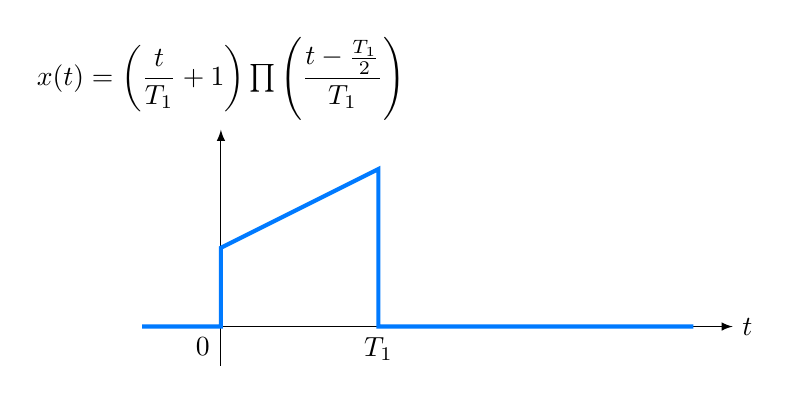
\begin{tikzpicture}[>=latex]
                \draw[->] (-1, 0) -- (6.5,0) node[right] {$t$};
                \draw[->] (0,-0.5) -- (0, 2.5) node[above] {$x(t)=\left( \dfrac{t}{T_1}+1 \right ) \prod\left( \dfrac{t-\frac{T_1}{2} }{T_1} \right )$};
                \draw[lightblue, line width=1.5] (-1,0) -- (0,0) node[below left, black] {$0$} -- (0,1) -- (2,2) -- (2,0) node[below, black] {$T_1$} -- (6,0);
              \end{tikzpicture}
            \end{center}
          \end{itemize}
        \item Segunda señal: \[
        h(t)=\prod\left( \dfrac{t-\frac{T_2}{2} }{T_2} \right) .
        \] 
        \begin{itemize}[label=\textbullet]
          \item Esta es una función rectangular centrada en $t=\dfrac{T_2}{2}$ con un ancho de $T_2$. Es igual a 1 en el intervalo $[0,T_2]$ y 0 fuera de este intervalo.
            \begin{center}
              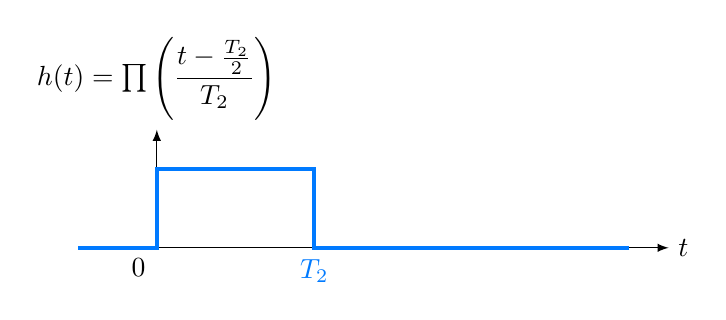
\begin{tikzpicture}[>=latex]
                \draw[->] (-1,0) -- (6.5,0) node[right] {$t$};
                \draw[->] (0,0.5) -- (0,1.5) node[above] {$h(t)=\prod\left( \dfrac{t-\frac{T_2}{2} }{T_2} \right )$};
                \draw[lightblue, line width=1.5] (-1,0) -- (0,0) node[below left, black] {$0$} -- (0,1) -- (2,1) -- (2,0) node[below] {$T_2$} -- (6,0);
              \end{tikzpicture}
            \end{center}
        \end{itemize}
      \item Convolución de las señales

        La convolución de $x(t)$ y  $h(t)$ se define como:  \[
        y(t)=(x\ast h)(t)=\int_{-\infty}^{\infty} x(\tau)h(t-\tau) \mathrm{d}\tau.
        \] 
        Dado que $x(t)$ está definido en  $[0,T_1]$ y $h(t)$ en  $[0,T_2]$, la convolución será no nula únicamente en el intervalo donde ambas funciones se superponen. Esto ocurre en el intervalo $[0,T_1+T_2]$.

        \textbf{Intervalo de integración:}
        \begin{itemize}[label=\textbullet]
          \item Para cada $t\in [0,T_1+T_2]$, la integral se reduce a: \[
          y(t)=\int_{\max(0,t-T_2)}^{\min(T_1,t)}  x(\tau)\mathrm{d}\tau,
        \] ya que $h(t-\tau)$ es no nula cuando  $t-\tau\in [0,T_2]$, es decir, $\tau\in [t-T_2,t]$, y $x(\tau)$ es no nula solo cuando  $\tau\in (0,T_1)$.
        \end{itemize}
        \end{itemize}
      \item Evaluar la integral

        En el interalo de integración, $x(\tau)=\dfrac{\tau}{T_1}+1$. Sustituyendo esto en la integral: \[
          \begin{aligned}
          y(t)=\int_{\max(0,t-T_2)}^{\min(T_1,t)} \left( \dfrac{\tau}{T_1}+1 \right) \mathrm{d}\tau&=\int_{\max(0,t-T_2)}^{\min(T_1,t)} \dfrac{\tau}{T_1}\mathrm{d}\tau+\int_{\max(0,t-T_2)}^{\min(T_1,t)} 1\mathrm{d}\tau\\ &=\bboxed{\dfrac{1}{T_1}\left( \dfrac{\min(T_1,t)^2}{2}-\dfrac{\max(0,t-T_2)^2}{2} \right ) +\min(T_1,t)-\max(0,t-T_2)} 
          \end{aligned}
        \] 
         \begin{itemize}[label=\textbullet]
           \item $\int_{\max(0,t-T_2)}^{\min(T_1,t)} \dfrac{\tau}{T_1}\mathrm{d}\tau=\dfrac{1}{T_1}\int_{\max(0,t-T_2)}^{\min(T_1,t)} \tau\mathrm{d}\tau=\dfrac{1}{T_1}\left[ \dfrac{\tau^2}{2} \right]_{\max(0,t-T_2)}^{\min(T_1,t)}=\dfrac{1}{T_1}\left( \dfrac{\min(T_1,t)^2}{2}-\dfrac{\max(0,t-T_2)^2}{2} \right)  $.
           \item $\int_{\max(0,t-T_2)}^{\min(T_1,t)} 1\mathrm{d}\tau = [\tau]_{\max(0,t-T_2)}^{\min(T_1,t)} =\min(T_1,t)-\max(0,t-T_2)$
        \end{itemize}
    \end{enumerate}
  \item \lb{Calcule la convolución de $x(t)=e^{2t}u(-t)$ con $h(t)=u(t-3)$.}

    La convolució se define como: \[
    y(t)=(x\ast h)(t)=\int_{-\infty}^{\infty} x(\tau)h(t-\tau)\mathrm{d}\tau 
    \] 
    \textbf{Análisis de las señales}
    \begin{itemize}[label=\textbullet]
      \item $x(t)=e^{2t}u(-t) $ es una señal exponencial que existe solo para $t<0$.
      \item  $h(t)=u(t-3)$ es un escalón unitario desplazado 3 unidades a la derecha.
    \end{itemize}
    \begin{center}
      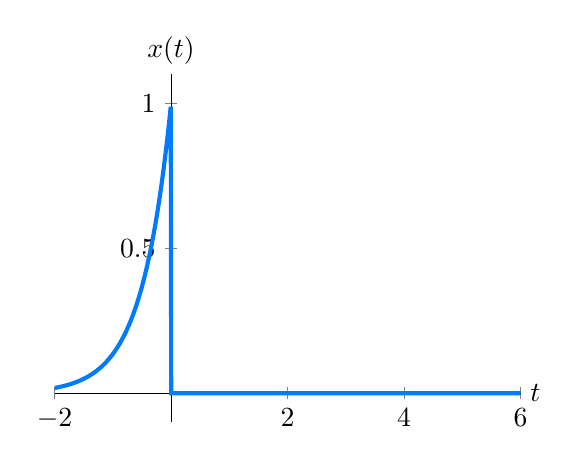
\begin{tikzpicture}
          \begin{axis}[
              width=7.5cm,
              height=6cm,
              axis lines=middle,
              xlabel={$t$},
              ylabel={$x(t)$},
              ymin=-0.1, ymax=1.1,
              axis line style={-},
		  xlabel style={at={(axis cs:6,0)}, anchor=west},
        ylabel style={at={(axis cs:0,1.1)}, anchor=south},
          ]
              \addplot[
                  domain=-2:6,
                  samples=1000,
                  lightblue, line width=1.5
              ]
              {exp(2*x)*(x<=0)};
          \end{axis}
      \end{tikzpicture}\qquad
      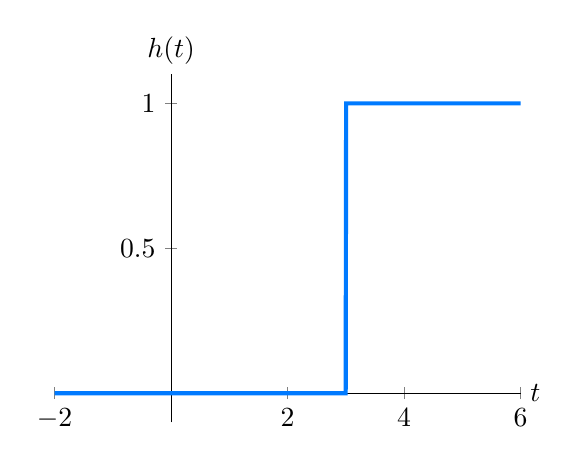
\begin{tikzpicture}
          \begin{axis}[
              width=7.5cm,
              height=6cm,
              axis lines=middle,
              xlabel={$t$},
              ylabel={$h(t)$},
              ymin=-0.1, ymax=1.1,
              axis line style={-},
              xlabel style={at={(axis cs:6,0)}, anchor=west},
        ylabel style={at={(axis cs:0,1.1)}, anchor=south},
          ]
              \addplot[
                  domain=-2:6,
                  samples=1000,
                  lightblue, line width=1.5
              ]
              {x>=3 ? 1 : 0};
          \end{axis}
      \end{tikzpicture}
    \end{center}
    \textbf{Determinación de los límites de integración}
    
    Para que la integral no sea nula, necesitamos que:
    \begin{itemize}[label=\textbullet]
      \item $\tau<0$ (debido a $u(-\tau)$ en  $x(\tau)$) 
      \item $t-\tau>3$ (debido a $u(t-\tau-3)$ en  $h(t-\tau)$)
    \end{itemize}
    De $t-\tau>3$, obtenemos:  $\tau<t-3$. Por tanto, los límites de itengración son:
     \begin{itemize}[label=\textbullet]
      \item Límite inferior: $-\infty$
      \item Límite superior: $\min(0,t-3)$
    \end{itemize}
    \textbf{Cálculo de la convolución}
    \[
    y(t)=\int_{-\infty}^{\min(0,t-3)} e^{2\tau}(u-\tau)u(t-\tau-3)\mathrm{d}\tau 
    \] 
    Debemos considerar dos casos:
    \begin{enumerate}[label=Caso \arabic*:]
      \item $t<3$

        En este caso,  $t-3<0$, por lo que  $\min(0,t-3)=t-3$
         \[
        y(t)=\int_{-\infty}^{t-3} e^{2\tau}\mathrm{d}\tau=\dfrac{1}{2}e^{2(t-3)}=\dfrac{1}{2}e^{2t-6}    
        \] 
      \item $t\ge 3$

        En este caso, $t-3\ge 0$, por lo que $\min(0,t-3)=0$
         \[
           y(t)=\int_{-\infty}^{0} e^{2\tau}\mathrm{d}\tau=\dfrac{1}{2}
        \] 
        La convolución es: \[
        y(t)=\begin{cases}
          \dfrac{1}{2}e^{2t-6}, & t<3\\
          \dfrac{1}{2}, & t\ge 3
        \end{cases}
        \] 
        \begin{center}
          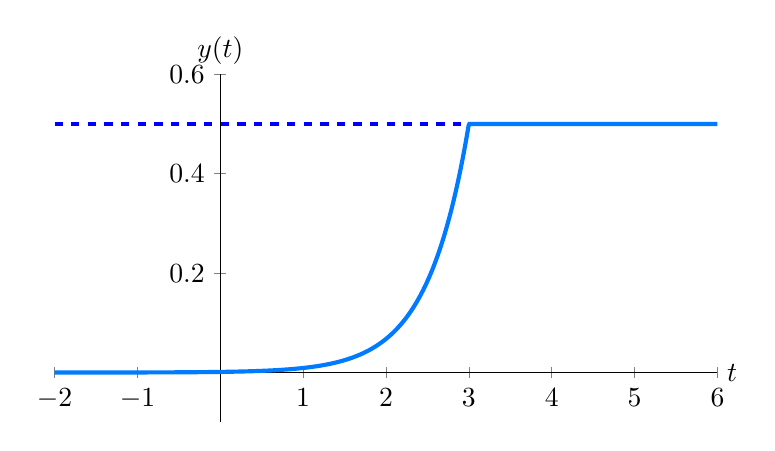
\begin{tikzpicture}
            \begin{axis}[
              width=10cm,
              height=6cm,
              axis lines=middle,
              xlabel={$t$},
              ylabel={$y(t)$},
              axis line style={-},
              ymin=-0.1, ymax=0.6,
              every axis plot/.append style={line width=1.5, lightblue},
		  xlabel style={at={(axis cs:6,0)}, anchor=west},
        ylabel style={at={(axis cs:0,0.6)}, anchor=south},
              ]
              \addplot[domain=-2:6, samples=1000] {x < 3 ? 0.5*exp(2*x-6) : 0.5};
              \addplot[blue, dashed, domain=-2:3, samples=2] {0.5};
            \end{axis} 
          \end{tikzpicture}
        \end{center}
    \end{enumerate}
  \item \lb{Sea $x[n]=\delta[n]+2\delta[n-1]-\delta[n-3]$ y  $h[n]=2\delta[n+1]+2\delta[n-1]$} 
    \begin{center}
      \begin{tikzpicture}[>=latex]
        \draw[->] (-1,0) -- (6,0) node[right] {$n$};
        \draw[->] (0,-1) -- (0,2.1) node[above] {$x[n]$};
        \draw[-*, lightblue, line width=1.2] (0,0) -- (0,1);
        \draw[-*, lightblue, line width=1.2] (1,0) -- (1,2);
        \draw[-*, lightblue, line width=1.2] (3,0) -- (3,-1);
        \foreach \x/\n in {-1/0, 2/0, 4/0, 5/0} {
        \fill[lightblue] (\x,\n) circle (3pt);
        }
      \end{tikzpicture}\qquad
      \begin{tikzpicture}[>=latex]
        \draw[->] (-1,0) -- (6,0) node[right] {$n$};
        \draw[->] (0,-1) -- (0,2.1) node[above] {$h[n]$};
        \foreach \x/\n in {-1/2,0/0,1/2,2/0,3/0,4/0,5/0} {
          \fill[lightblue] (\x,\n) circle (3pt);
        }
        \foreach \x in {-1,1} {\draw[lightblue, line width=1.5] (\x,0) -- (\x,2);}
      \end{tikzpicture}
    \end{center}
    \begin{enumerate}[label=\color{red}\textbf{\alph*)}]
      \item \db{$y_1=x[n]\ast h[n]$} 
       
        La convolución se calcula como: \[
          y_1=\sum_{k=-\infty}^{\infty} x[k]h[n-k]
        \] 
        Sustituyendo $x[k]$ y  $h[n-k]$, tenemos: \[
          y_1[n]=x[0]h[n]+x[1]h[n-1]+x[3]h[n-3]
        \] 
         \begin{itemize}[label=\textbullet]
           \item $x[0]=1\longrightarrow h[n]=2\delta[n+1]+2\delta[n-1]$
           \item $x[1]=2\longrightarrow h[n-1]=2\delta[n]+2\delta[n-2]$
           \item $x[3]=-1\longrightarrow h[n-3]=2\delta[n-2]+2\delta[n-4]$
        \end{itemize}
        Sumando todas las contribuciones: \[
          y_1[n]=2\delta[n+1]+2\delta[n-1]+4\delta[n]+4\delta[n-2]-2\delta[n-2]-2\delta[n-4]=2\delta[n+1]+4\delta[n]+2\delta[n-1]+2\delta[n-2]-2\delta[n-4]
        \] 
        \begin{center}
          \begin{tikzpicture}[>=latex]
            \draw[->] (-1,0) -- (6,0) node[right] {$n$};
            \draw[->] (0,-2) -- (0,4.1) node[above] {$y_1[n]$};
            \foreach \x/\n in {-1/2,0/4,1/2,2/2,3/0,4/-2,5/0} {
              \draw (\x, 0.1) -- (\x,-0.1) node[below] {$\x$};
              \draw[line width=1.5, lightblue] (\x,0) -- (\x,\n);
              \fill[lightblue] (\x,\n) circle (3pt);
            }
          \end{tikzpicture}
        \end{center}
      \item \db{$y_2[n]=x[n+2]\ast h[n]$}
        
        Señal desplazada: \[
          x[n+2]=\delta[n+2]+2\delta[n+1]-\delta[n-1]
        \] 
        La convolución se calcula como: \[
          y_2[n]=\sum_{k=-\infty}^{\infty} x[k+2]h[n-k]
        \] 
        Sustituyendo $x[k+2]$ y  $x[n-k]$, tenemos:  \[
          y_2[n]=x[-2]h[n+2]+x[-1]h[n+1]+x[1]h[n-1]
        \] 
        \begin{itemize}[label=\textbullet]
          \item $x[-2]=1\longrightarrow h[n+2]=2\delta[n+3]+2\delta[n+1]$
          \item $x[-1]=2\longrightarrow h[n+1]=2\delta[n+2]+2\delta[n]$
          \item $x[1]=-1\longrightarrow h[n-1]=2\delta[n]+2\delta[n-2]$
        \end{itemize}
        Sumando todas las contribuciones: \[
          y_2[n]=2\delta[n+3]+2\delta[n+1]+4\delta[n+2]+4\delta[n]-2\delta[n]-2\delta[n-2]=2\delta[n+3]+4\delta[n+2]+2\delta[n+1]+2\delta[n]-2\delta[n-2]
        \] 
        \begin{center}
          \begin{tikzpicture}[>=latex]
            \draw[->] (-4,0) -- (5,0) node[right] {$n$};
            \draw[->] (0,-2) -- (0,4.1) node[above] {$y_2[n]$};
            \foreach \x/\n in {-4/0,-3/2,-2/4,-1/2,0/2,1/0,2/-2, 3/0, 4/0} {
              \draw (\x,0.1) -- (\x,-0.1) node[below] {$\x$};
              \draw[line width=1.5, lightblue] (\x,0) -- (\x,\n);
              \fill[lightblue] (\x,\n) circle (3pt);
            }
          \end{tikzpicture}
        \end{center}
      \item \db{$y_3[n]=x[n]\ast h[n+2]$} 

        Señal desplazada: \[
          h[n+2]=2\delta[n+3]+2\delta[n+1]
        \] 
        La convolución se calcula como: \[
          y_3[n]=\sum_{k=-\infty}^{\infty} x[k]h[n-k+2]
        \] 
        Sustituyendo $x[k]$ y $h[n-k+2]$, tenemos:  \[
          y_3[n]=x[0]h[n+2]+x[1]h[n+1]+x[3]h[n-1]
        \] 
        \begin{itemize}[label=\textbullet]
          \item $x[0]=1\longrightarrow h[n+2]=2\delta[n+3]+2\delta[n+1]$
          \item $x[1]=2\longrightarrow h[n+1]=2\delta[n+2]+2\delta[n]$
          \item $x[3]=-1\longrightarrow h[n-1]=2\delta[n]+2\delta[n-2]$
        \end{itemize}
        Sumando todas las contribuciones:
        \[
          y_3[n]=2\delta[n+3]+2\delta[n+1]+4\delta[n+2]+4\delta[n]-2\delta[n]-2\delta[n-2]=2\delta[n+3]+4\delta[n+2]+2\delta[n+1]+2\delta[n]-2\delta[n-2]
        \] 
        \begin{center}
          \begin{tikzpicture}[>=latex]
            \draw[->] (-4,0) -- (5,0) node[right] {$n$};
            \draw[->] (0,-2) -- (0,4.1) node[above] {$y_3[n]$};
            \foreach \x/\n in {-4/0,-3/2,-2/4,-1/2,0/2,1/0,2/-2, 3/0, 4/0} {
              \draw (\x,0.1) -- (\x,-0.1) node[below] {$\x$};
              \draw[line width=1.5, lightblue] (\x,0) -- (\x,\n);
              \fill[lightblue] (\x,\n) circle (3pt);
            }
          \end{tikzpicture}

        \end{center}
    \end{enumerate}
  \item \lb{Un sistema lineal $S$ relaciona su entrada  $x[n]$ y su salida $y[n]$ como \[
        y[n]=\sum_{k=-\infty}^{\infty} x[k]g[n-2k]
    \] donde $g[n]=u[n]-u[n-4]$.} 
    \begin{enumerate}[label=\color{red}\textbf{\alph*)}]
      \item \db{Determine $y[n]$ cuando $x[n]=\delta[n-1]$} 

        La relación entre la entrada y la salida está dada por: \[
          y[n]=\sum_{k=-\infty}^{\infty} x[k]g[n-2k]
        \] 
        Sustituyendo $x[n]=\delta[n-1]$, sabemos que  $\delta[n-1]$ es no nula cuando  $n=1$. Por lo tanto, la suma se reduce a:  \[
          y[n]=g[n-2(1)]=g[n-2]
        \] 
        Dado que $g[n]=u[n]-u[n-4]$, tenemos:  \[
          g[n-2]=u[n-2]-u[n-6]
        \] 
        Por lo tanto: \[
          y[n]=u[n-2]-u[n-6]
        \] 
        Esto significa que $y[n]$ es un pulso rectangular que comienza en  $n=2$ y termina en  $n=5$ (ya que $u[n-6]$) se activa en $n=6$.
         \begin{center}
           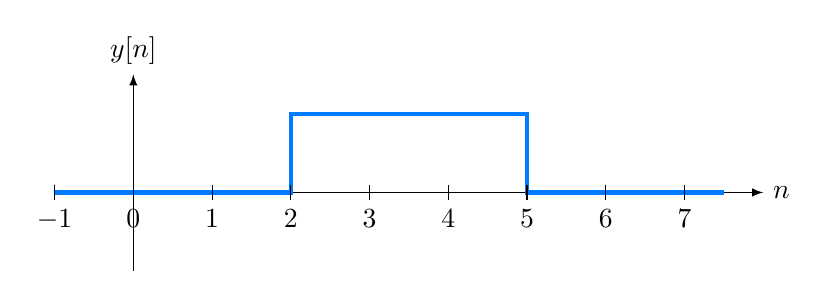
\begin{tikzpicture}[>=latex]
            \draw[->] (-1,0) -- (8,0) node[right] {$n$};
            \draw[->] (0,-1) -- (0,1.5) node[above] {$y[n]$};
            \draw[lightblue, line width=1.5] (-1,0) -- (2,0) -- (2,1) -- (5,1) -- (5,0) -- (7.5,0); 
            \foreach \x in {-1,0,...,7} {\draw (\x,0.1) -- (\x,-0.1) node[below] {$\x$};}
          \end{tikzpicture}
        \end{center}
      \item \db{Determine $y[n]$ cuando $x[n]=\delta[n-2]$} 

        De nuevo, la relación es: \[
          y[n]=\sum_{k=-\infty}^{\infty} x[k]g[n-2k]
        \] 
        Sustituyendo $x[n]=\delta[n-2]$, sabemos que  $\delta[n-2]$ es no nula solo cuando  $n=2$. Por lo tanto, la suma se reduce a: \[
          y[n]=g[n-2(2)]=g[n-4]
        \] 
        Dado que $g[n]=u[n]-u[n-4]$, tenemos:  \[
          g[n-4]=u[n-4]-u[n-8]
        \] 
        Esto significa que $y[n]$ es un pulso rectangular que comienza en $n=4$ y termina en $n=7$ (ya que $u[n-8]$ se activa en $n=8$)
        \begin{center}
           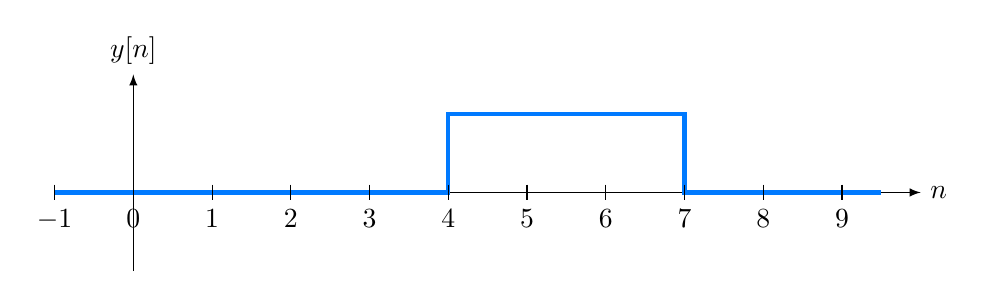
\begin{tikzpicture}[>=latex]
            \draw[->] (-1,0) -- (10,0) node[right] {$n$};
            \draw[->] (0,-1) -- (0,1.5) node[above] {$y[n]$};
            \draw[lightblue, line width=1.5] (-1,0) -- (4,0) -- (4,1) -- (7,1) -- (7,0) -- (9.5,0); 
            \foreach \x in {-1,0,...,9} {\draw (\x,0.1) -- (\x,-0.1) node[below] {$\x$};}
          \end{tikzpicture}
        \end{center}

      \item \db{¿Es $S$ un sistema LTI?} 

        Para determinar si el sitema es \textbf{lineal} e \textbf{invariante} en el tiempo, evaluamos cada propiedad:
        \begin{itemize}[label=\textbullet]
          \item \textbf{Linealidad:}

            Un sistema es lineal si satisface el principio de superposición, es decir, si para dos entradas $x_1[n]$ y $x_2[n]$ con salidas $y_1[n]$ y $y_2[n]$, respectivamente, se cumple que: \[
              S \{ax_1[n]+bx_2[n]\} =ay_1[n]+by_2[n]
            \] 
            En este caso, la salida está dada por una suma ponderada de $x[k]$ y  $g[n-2k]$, lo cual es una operación lineal. Por lo tanto, el sistema es  \textbf{lineal}.
          \item \textbf{Invanrianza en el tiempo:}

            Un sistema es invariante en el tiempo si un desplazamiento en la entrada produce el mismo desplazamiento en la salida. Es decir, si para una entrada $x[n]$ con salida  $y[n]$, al desplazar la entrada  $x[n-n_0]$, la salida se desplaza de manera idéntica $y[n-n_0]$.

            En este caso, la salida depende de $g[n-2k]$, que introduce un factor de escalamiento en el índice  $k$. Esto significa que el sistema  \textbf{no es invariante en el tiempo}, ya que el desplazamiento de la entrada no se traduce directamente en un desplazamiento de la salida. 
        \end{itemize}
      \item \db{Determine $y[n]$ cuando $x[n]=u[n]$} 

        De nuevo, la relación es: \[
          y[n]=\sum_{k=-\infty}^{\infty} x[k]g[n-2k]
        \] 
        Sustituyendo $x[n]=u[n]$, sabemos que  $u[n]$ es no nula para  $k\ge 0$. Por lo tanto, la suma se reduce a: \[
          y[n]=\sum_{k=0}^{\infty} g[n-2k]
        \] 
        Dado que $g[n]=u[n]-u[n-4]$, tenemos:  \[
          g[n-2k]=u[n-2k]-u[n-2k-4]
        \] 
        Sustituyendo esto en la suma: \[
          y[n]=\sum_{k=0}^{\infty} (u[n-2k]-u[n-2k-4])
        \] 
        La suma se puede interpretar como una superposición de pulsos rectangulares desplazados. Cada término $u[n-2k]-u[n-2k-4]$ es un pulso rectangular de longitud 4, comenzando en  $n=2k$ y terminando en  $n=2k+3$.

        Por lo tanto,  $y[n]$ es una secuencia de pulsos rectangulares de longitud 4, comenzando en  $n=0$ y repitiéndose cada 2 unidades de tiempo.
         \begin{center}
           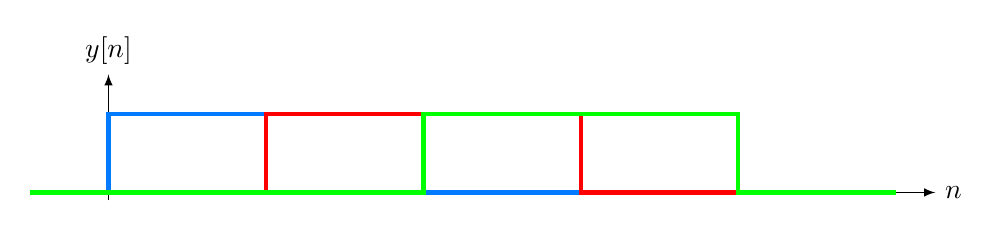
\begin{tikzpicture}[>=latex]
            \draw[->] (-1,0) -- (10.5,0) node[right] {$n$};
            \draw[->] (0,-0.1) -- (0, 1.5) node[above] {$y[n]$};
            \draw[lightblue, line width=1.5] (-1,0) -- (0,0) -- (0,1) -- (4,1) -- (4,0) -- (10, 0);
            \draw[red, line width=1.5] (-1,0) -- (2,0) -- (2,1) -- (6,1) -- (6,0) -- (10, 0);
            \draw[green, line width=1.5] (-1,0) -- (4,0) -- (4,1) -- (8,1) -- (8,0) -- (10, 0);
          \end{tikzpicture}
        \end{center}
    \end{enumerate}
  \item \lb{Determine y esboce la convolución de las siguientes señales: \[
  \begin{array}{cc}
    x(t)=\begin{cases}
      t+1, & 0\le t\le 1\\
      2-t, & 1<t\le 2\\
      0, & \text{otro valor}
    \end{cases} & h(t)=\delta(t+2)+2\delta(t+1)
  \end{array}
\] }
La convolución de dos señales $x(t)$ y  $h(t)$ está definida como:  \[
y(t)=(x\ast h)(t)=\int_{-\infty}^{\infty} h(\tau)h(t-\tau)\mathrm{d}\tau 
\] 
En este caso:
\begin{itemize}[label=\textbullet]
  \item $x(t)$ es una función triangular definida por tramos:  \[
  x(t)=\begin{cases}
    t+1, & 0\le t\le 1\\
    2-t, & 1<t\le 2\\
    0, & \text{en otro caso}
  \end{cases}
  \] 
\item $h(t)$ es una combinación de deltas desplazadas:  \[
h(t)=\delta(t+2)+2\delta(t+1)
\] 
\end{itemize}
Dado que $h(t)$ está compuesto por deltas, la convolución se simplifica porque las deltas actúan como "muestradoras" de  $x(t)$. Específicamente, la convolución se convierte en:  \[
y(t)=x(t)\ast h(t)=x(t+2)+2x(t+1)
\] 
\begin{enumerate}[label=Paso \arabic*:]
  \item Determinar $x(t+2)$

    Para obtener  $x(t+2)$, desplazamos  $x(t)$ dos unidades hacia la izquierda. Esto significa que el soporte de  $x(t+2)$ (el intervalo donde es cero) será:  \[
    -2\le t\le -1
    \] 
    En este intervalo, la forma de $x(t+2)$ es: 
    \begin{itemize}[label=\textbullet]
      \item Para $-2\le t\le -1,x(t+2)=t+2+1=t+3$.
    \end{itemize}
    Por lo tanto: \[
    x(t+2)=\begin{cases}
      t+3, & -2\le t\le -1\\
      0, & \text{en otro caso}
    \end{cases}
    \] 
  \item Determinar $2x(t+1)$

    Para obtener  $2x(t+1)$, desplazamos  $x(t)$ una unidad hacia la izquierda y multiplicamos por 2. Esto significa que el soporte de  $2x(t+1)$ será:  \[
    -1\le t\le 1
    \] 
    En este intervalo, la forma de $x(t+1)$ es:
     \begin{itemize}[label=\textbullet]
      \item Para $-1\le t\le 0,x(t+1)=t+1+1=t+2$
      \item Para $0<t\le 1,x(t+1)=2-(t-1)=1-t$
    \end{itemize}
    Multiplicando por 2, obtenemos: \[
    2x(t+1)=\begin{cases}
      2(t+2)=2t+4, & -1\le t\le 0\\
      2(1-t)=2-2t, & 0<t\le 1\\
      0, & \text{en otro caso}
    \end{cases}
    \] 
  \item Sumar $x(t+2)$ y  $2x(t+1)$

    Ahora sumamos las dos contribuciones  $x(t+2)$ y  $2x(t+1)$. El soporte total de $y(t)$ será la unión de los soportes de  $x(t+2)$ y  $2x(t+1)$, es decir:  \[
    -2\le t\le 1
    \] 
    Dividimos el cálculo en intervalos:
    \begin{itemize}[label=\textbullet]
      \item Para $-2\le t<-1$:
        \begin{itemize}[label=\textbullet]
          \item $x(t+2)=t+3$
          \item  $2x(t+1)=0$ (porque $t+1<-1$) 
          \item $y(t)=t+3$
        \end{itemize}
      \item Para $-1\le t<0$:
        \begin{itemize}[label=\textbullet]
          \item $x(t+2)=t+3$
          \item  $2x(t+1)=2t+4$
          \item  $y(t)=(t+3)+(2t+4)=3t+7$
        \end{itemize}
      \item Para $0\le t\le 1$:
        \begin{itemize}[label=\textbullet]
          \item $x(t+2)=0$ (porque $t+2>2$) 
          \item $2x(t+1)=2-2t$
          \item  $y(t)=0+(2-2t)=2-2t$
        \end{itemize}
    \end{itemize}
\end{enumerate}
    La salida $y(t)$ es:  \[
    y(t)=\begin{cases}
      t+3, & -2\le t<-1\\
      3t+7, & -1\le t<0\\
      2-2t, & 0\le t<1\\
      0, & \text{en otro caso}
    \end{cases}
    \]
    \begin{center}
      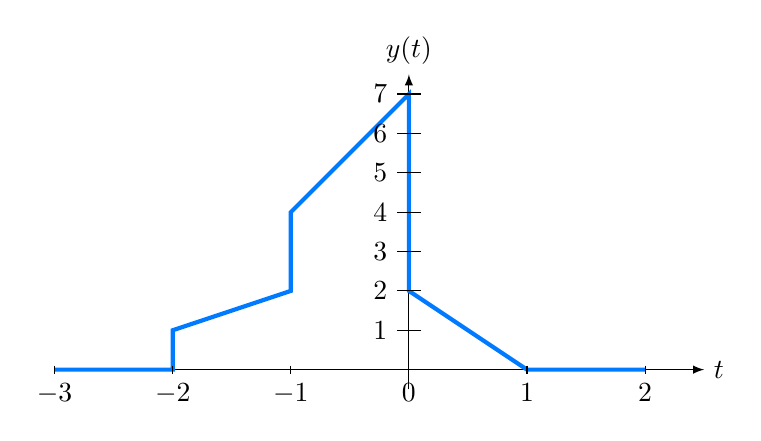
\begin{tikzpicture}[>=latex, yscale=0.5, xscale=1.5]
        \draw[->] (-3,0) -- (2.5, 0) node[right] {$t$};
        \draw[->] (0,-0.5) -- (0,7.5) node[above] {$y(t)$};
        \draw[lightblue, line width=1.5] (-3,0) -- (-2,0) -- (-2,1) -- (-1,2) -- (-1, 4) -- (0,7) -- (0,2) -- (1,0) -- (2,0);
        \foreach \x in {-3, -2, ..., 2} {\draw (\x,0.1) -- (\x,-0.1) node[below] {$\x$};}
          \foreach \y in {1,...,7} {\draw (0.1,\y) -- (-0.1,\y) node[left] {$\y$};}
      \end{tikzpicture}
    \end{center}
  \item \lb{Sean \[
  x(t)=\begin{cases}
    1, & 0\le t\le 1\\
    0,  & \text{otro valor}
  \end{cases}\qquad h(t)=x\left( \dfrac{t}{\alpha} \right),\text{ donde $0<\alpha\le 1$ }
  \] } 
  \begin{enumerate}[label=\color{red}\textbf{\alph*)}]
    \item \db{Determine y esboce $y(t)=x(t)\ast h(t)$.}

      La convolución de $x(t)$ y  $h(t)$ está definida como:  \[
      y(t)=(x\ast h)(t)=\int_{-\infty}^{\infty} x(\tau)h(t-\tau)\mathrm{d}\tau 
      \] 
      Dado que $x(t)$ es una función rectangular definida como:  \[
      x(t)=\begin{cases}
        1, & 0\le t\le 1\\
        0, & \text{en otro caso}
      \end{cases}
      \] 
      y que $h(t)=x\left( \dfrac{t}{\alpha} \right) $, podemos escribir $h(t)$ como:  \[
      h(t)=\begin{cases}
        1, & 0\le \dfrac{t}{\alpha}\le 1\\
        0, & \text{en otro caso}
        \end{cases} \begin{array}{l}
        \longrightarrow 0\le t\le \alpha\\
        \\
      \end{array}
      \] 
      Por lo tanto: \[
      h(t)=\begin{cases}
        1, & 0\le t\le \alpha\\
        0, & \text{en otro caso}
      \end{cases}
      \] 
      Ambas señales son rectángulos, y la convolución de dos rectángulos es un triángulo. El soporte de $y(t)$ será la suma de los soporte de  $x(t)$ y $h(t)$, es decir:  \[
        \text{Soporte de }y(t):\quad [0,1+\alpha]
      \] 
      \textbf{Cálculo de $y(t)$:} 

      La convolución se calcula como: $$y(t)=\int_{-\infty}^{\infty} x(\tau)h(t-\tau)\mathrm{d}\tau $$
      Dado que $x(\tau)$ y  $h(t-\tau)$, son no nula en los intervalos  $[0,1]$ y  $[t-\alpha,t]$, respectivamente, la integral se reduce al intervalo donde ambos se solapan. Esto depende del valor de $t$:
       \begin{itemize}[label=\textbullet]
        \item \textbf{Para $0\le t\le \alpha$:}

          En este caso, el solapamiento ocurre en $[0,t]$. Por lo tanto:  \[
            y(t)=\int_{0}^{t} 1\cdot 1\mathrm{d}\tau=[\tau]_0^t=t 
          \] 
        \item \textbf{Para $\alpha\le t\le 1$:} 

          En este caso, el solapamiento ocurre en $[t-\alpha,t]$. Por lo tanto: \[
            y(t)=\int_{t-\alpha}^{t} 1\cdot 1\mathrm{d}\tau=[\tau]_{t-\alpha}^{t}=t-(t-\alpha)=\alpha 
          \] 
        \item \textbf{Para $1<t\le 1+\alpha$:}

          En este caso, el solapamiento ocurre en $[t-\alpha,1]$. Por lo tanto: \[
            y(t)=\int_{t-\alpha}^{1} 1\cdot 1\mathrm{d}\tau=[\tau]_{t-\alpha}^1=1-(t-\alpha)=1+\alpha-t 
          \] 
        \item \textbf{Para $t>1+\alpha$:} 

          No hay solapamiento, por lo que: \[
          y(t)=0
          \] 
      \end{itemize}
      La salida $y(t)$ es:  \[
      y(t)=\begin{cases}
        t, & 0\le t\le \alpha\\
        \alpha, & \alpha<t\le 1\\
        1+\alpha-t, & 1<t\le 1+\alpha\\
        0, & \text{en otro caso}
      \end{cases}
      \] 
      Esto corresponde a un triángulo con base en $[0,1+\alpha]$, que crece linealmente en $[0,\alpha]$, se mantiene constante en $[\alpha,1]$, y decrece linealmente en $[1,1+\alpha]$.
      \begin{center}
        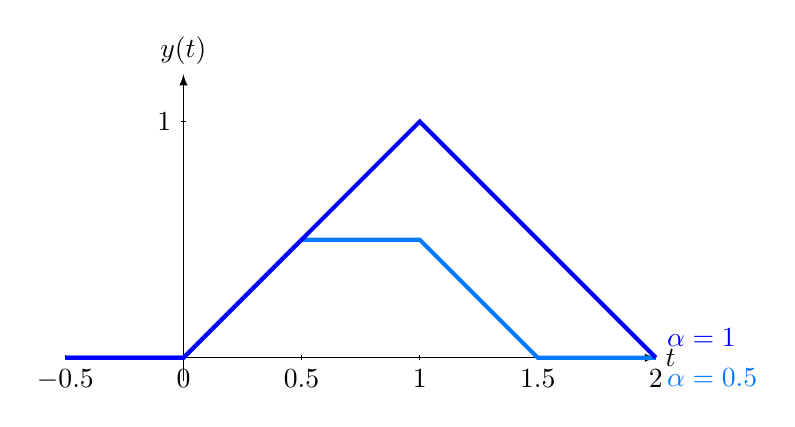
\begin{tikzpicture}[>=latex, scale=3]
          \draw[->] (-0.5, 0) -- (2,0) node[right] {$t$};
          \draw[->] (0,-0.1) -- (0,1.2) node[above] {$y(t)$};
          \foreach \x in {-0.5, 0, 0.5, ..., 2} {\draw (\x, 0.01) -- (\x,-0.01) node[below] {$\x$};}
          \draw[lightblue, line width=1.5] (-0.5,0) -- (0,0) -- (0.5,0.5) -- (1,0.5) -- (1.5,0) -- (2,0) node[below right] {$\alpha=0.5$};
          \draw[blue, line width=1.5] (-0.5,0) -- (0,0) -- (1,1) -- (2,0) node[above right] {$\alpha=1$};
          \draw (0.01,1) -- (-0.01,1) node[left] {$1$};
        \end{tikzpicture}
      \end{center}
    \item \db{Si $\dfrac{\mathrm{d}y(t)}{\dt}$ contiene sólo tres discontinuidades, ¿cuál es el valor de $\alpha$?} 

        La derivada de $y(t)$ seá: 
         \begin{itemize}[label=\textbullet]
            \item Para $0\le t\le \alpha,\,y(t)=t$, por lo que: \[
            \dfrac{\mathrm{d}y(t)}{\dt}=1
            \] 
        \item Para $\alpha<t\le 1,y(t)=\alpha$, por lo que: \[
        \dfrac{\mathrm{d}y(t)}{\dt}=0
        \] 
    \item Para $1<t\le 1+\alpha,y(t)=1+\alpha-t$, por lo que: \[
    \dfrac{\mathrm{d}y(t)}{\dt}=-1
    \] 
\item Para $t>1+\alpha,y(t)=0$, por lo que: \[
\dfrac{\mathrm{d}y(t)}{\dt}=0
\] 
        \end{itemize}
        Las discontinuidades en $\dfrac{\mathrm{d}y(t)}{\dt}$ ocurren en los puntos donde $y(t)$ cambia de pendiente. Estos puntos son:
         \begin{itemize}[label=\textbullet]
            \item En $t=\alpha$, donde la pendiente cambia de $1$ a $0$.
            \item En $t=1$, donde la pendiente cambia de $0$ a $-1$.
            \item En  $t=1+\alpha$, donde la pendiente cambia de $-1$ a  $0$.
        \end{itemize}
        Para que haya \textbf{solo tres discontinuidades}, los puntos $\alpha$  y $1+\alpha$ deben coincidir, es decir: \[
        \alpha=1+\alpha\longrightarrow \alpha=1.
        \] 
  \end{enumerate}
\item \lb{Sean \[
x(t)=u(t-3)-u(t-5)\qquad h(t)=e^{-3t} u(t)
\] } 
\begin{enumerate}[label=\color{red}\textbf{\alph*)}]
  \item \db{Calcule $y(t)=x(t)\ast h(t)$} 

      \textbf{Planteamiento}

      La convolución de $x(t)$ y  $h(t)$ está definida como:  \[
      y(t)=(x\ast h)(t)=\int_{-\infty}^{\infty} x(\tau)h(t-\tau)\mathrm{d}\tau 
      \] 
      Dado que:
      \begin{itemize}[label=\textbullet]
          \item $x(t)=u(t-3)-u(t-5)$, es un pulso rectangular definido en el intervalo  $[3,5]$.
          \item  $h(t)=e^{-3t}u(t) $, es una función exponencial decreciente que comienza en $t=0$
      \end{itemize}
      \begin{center}
          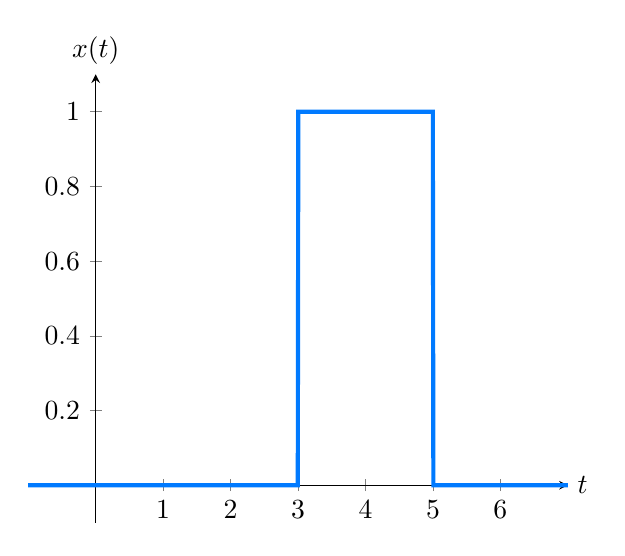
\begin{tikzpicture}
              \begin{axis}[
                  xmin= -1, xmax= 7,
                  ymin= -0.1, ymax = 1.1,
                  xlabel={$t$}, ylabel={$x(t)$},
						xtick={0,1,2,3,4,5,6},
                  axis lines = middle,
		  xlabel style={at={(axis cs:7,0)}, anchor=west},
        ylabel style={at={(axis cs:0,1.1)}, anchor=south},
              ]
                  \addplot[domain=-1:7, samples=1000, line width=1.5, lightblue]{x < 3 ? 0 : (x < 5 ? 1 : 0)};
              \end{axis}
          \end{tikzpicture}\qquad
				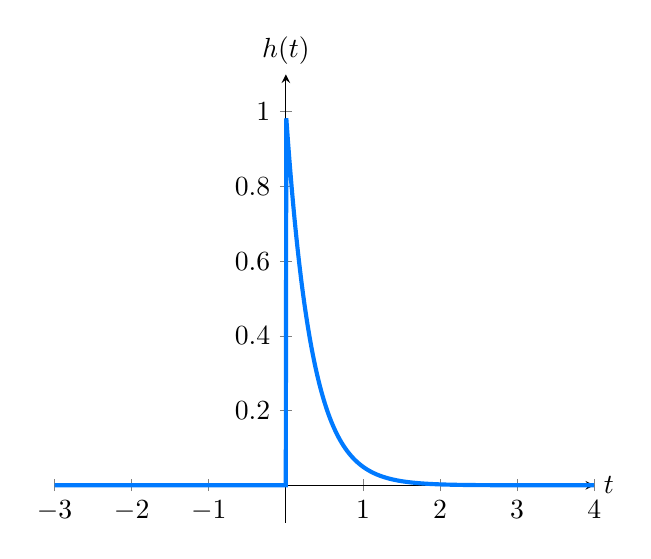
\begin{tikzpicture}
              \begin{axis}[
                  xmin= -3, xmax= 4,
                  ymin= -0.1, ymax = 1.1,
                  xlabel={$t$}, ylabel={$h(t)$},
                  axis lines = middle,
		  xlabel style={at={(axis cs:4,0)}, anchor=west},
        ylabel style={at={(axis cs:0,1.1)}, anchor=south},
              ]
                  \addplot[domain=-3:4, samples=1000, line width=1.5, lightblue]{x < 0 ? 0 : exp(-3*x)};
              \end{axis}
          \end{tikzpicture}
      \end{center}
      El soporte de $x(t)$ es  $[3,5]$, y el soporte de  $h(t)$ es  $[0,\infty)$. Por lo tanto, el soporte de  $y(t)$ será:  \[
          \text{Soporte de $y(t)$:}\quad[3,5+\infty)=[3,\infty).
      \] 
      \textbf{Cálculo de $y(t)$} 

      La convolución se evalúa en diferentes intervalos dependiendo del valor de $t$. Para  $t\ge 3$, el solapamiento entre $x(\tau)$ y  $h(t-\tau)$ ocurre en el intervalo  $[3,5]$. Por lo tanto, la integral se reduce a:  \[
      y(t)=\int_{3}^{5} h(t-\tau)\mathrm{d}\tau=\int_{3}^{5} e^{-3(t-\tau)}u(t-\tau)\mathrm{d}\tau.
      \] 
      El término $u(t-\tau)$ asegura que  $t-\tau\ge 0$, es decir, $\tau\le t$. Esto implica que el interalo de integración es: \[
          \tau\in [3,\min(5,t)]
      \] 
      Por lo tanto, el resultado depende de $t$:
       \begin{itemize}[label=\textbullet]
          \item \textbf{Para $3\le t<5$:}

              En este caso, $\min(5,t)=t$, y la integral se evalúa en  $[3,t]$:  \[
              y(t)=\int_{3}^{t} e^{-2(t-\tau)}\mathrm{d}\tau.  
              \] 
              Hacemos el cambio de variable $x=t-\tau$, lo que implica que  $\dx =\mathrm{d}\tau$. Los límites cambia de $\tau=3$ a  $\tau=t$, lo que da  $x=t-3$ a  $x=0$. La integral se convierte en:  \[
              y(t)=\int_{t-3}^{0} e^{-3x}(-\dx )=\int_{0}^{t-3}e^{-3x}\dx =\left[ \dfrac{e^{-3x} }{-3x} \right] _0^{t-3}=\dfrac{1}{3}\left( 1-e^{-3(t-3)}  \right).      
              \] 
          \item \textbf{Para $t\ge 5$:}

              En este caso, $\min(5,t)=5$, y la integral se evalúa en  $[3,5]$:  \[
              y(t)=\int_{3}^{5} e^{-3(t-\tau)}  \mathrm{d}\tau.
              \] 
              Usando el mismo cambio de variable $x=t-\tau$, con límites  $\tau=3$ a $\tau=5$, obtenemos $x=t-3$ a $x=t-5$. La integral se convierte en: \[
              y(t)=\int_{t-5}^{t-3}e^{-3x}\dx =\left[ \dfrac{e^{-3x} }{-3} \right]_{t-5}^{t-3}=\dfrac{1}{3}\left( e^{-3(t-5)}-e^{-3(t-3)}   \right)     .
              \] 
      \end{itemize}
      \textbf{Resultado final para $y(t)$} \[
      y(t)=\begin{cases}
          \dfrac{1}{3}(1-e^{-3(t-3)}), & 3\le t<5\\
          \dfrac{1}{3}\left( e^{-3(t-5)}-e^{-3(t-3)}   \right)  & t\ge 5
      \end{cases}
      \] 
      \begin{center}
          \begin{tikzpicture}
              \begin{axis}[
                  xmin= -1, xmax= 8,
                  ymin= -0.2, ymax = 0.4,
                  axis lines = middle,
                  xlabel={$t$}, ylabel={$y(t)$},
		  xlabel style={at={(axis cs:8,0)}, anchor=west},
        ylabel style={at={(axis cs:0,0.4)}, anchor=south},
              ]
                  \addplot[domain=3:5, samples=1000, lightblue, line width=1.5] {(1-exp(-3*(x-3)))/3};
                  \addplot[domain=5:8, samples=1000, lightblue, line width=1.5] {(exp(-3*(x-5))-exp(-3*(x-3)))/3};
              \end{axis}
          \end{tikzpicture}
      \end{center}
  \item \db{Calcule $g(t)=\dfrac{\mathrm{d}x(t)}{\dt}\ast h(t)$} 

      \textbf{Derivada de $x(t)$} 

      La derivada de $x(t)$ es: \[
      \dfrac{\mathrm{d}x(t)}{\dt}=\delta(t-3)-\delta(t-5).
      \] 
      Por lo tanto, la convolución $g(t)$ es:  \[
      g(t)=(\delta(t-3)-\delta(t-5))\ast h(t).
      \] 
          Usando la propiedad de desplazamiento de la convolución, sabemos que: \[
          \delta(t-t_0)\ast h(t)=h(t-t_0).
      \] 
      Por lo tanto: \[
      g(t)=h(t-3)-h(t-5).
      \] 
      Sustituyendo $h(t)=e^{-2t}u(t) $, tenemos: \[
          h(t-3)=e^{-3(t-3)}u(t-3),\quad h(t-5)=e^{-3(t-5)}u(t-5)  
      \] 
      Por lo tanto: \[
      g(t)=e^{-3(t-3)} u(t-3)-e^{-3(t-5)} u(t-5).
      \] 
      \begin{center}
          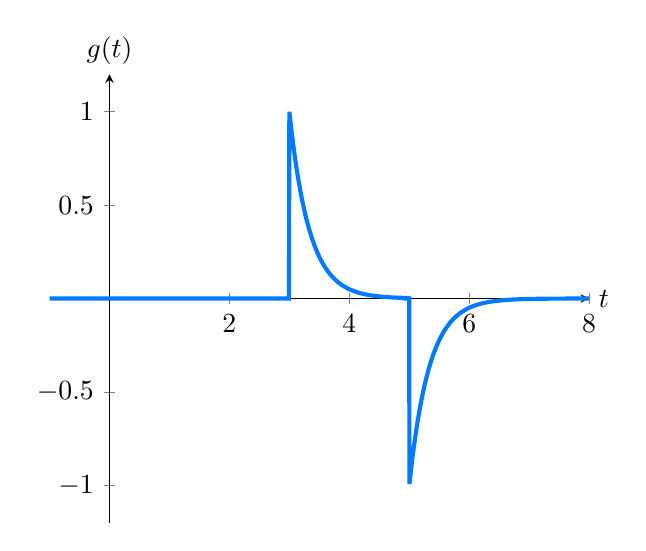
\begin{tikzpicture}
              \begin{axis}[
                  xmin= -1, xmax= 8,
                  ymin= -1.2, ymax = 1.2,
                  axis lines = middle,
						xlabel={$t$}, ylabel={$g(t)$},
		  xlabel style={at={(axis cs:8,0)}, anchor=west},
        ylabel style={at={(axis cs:0,1.2)}, anchor=south},
              ]
                  \addplot[domain=-1:5, samples=1000, lightblue, line width=1.5]{x<3 ? 0 : exp(-3*(x-3))};
                  \addplot[domain=4.9:8, samples=1000, lightblue, line width=1.5]{x<5 ? 0 : -exp(-3*(x-5))};
              \end{axis}
          \end{tikzpicture}
      \end{center}
  \item \db{Establece una relación entre $g(t)$ e $y(t)$} 

      Sabemos que $x(t)$ está relacionado con su derivada por:  \[
      x(t)=\int_{-\infty}^{t} \dfrac{\mathrm{d}x(\tau)}{\mathrm{d}\tau} \mathrm{d}\tau.
      \] 
      Por la propiedad de la convolución, esto implica que: \[
      y(t)=(x(t)\ast h(t))=\int_{-\infty}^{t} g(\tau)\mathrm{d}\tau .
      \] 
      En otras palabras, $y(t)$  \textbf{es la integral acumulativa de $g(t)$:} \[
      y(t)=\int_{-\infty}^{t} g(\tau)\mathrm{d}\tau. 
      \]  
\end{enumerate}
\item \lb{Calcule la convolución de los siguientes pares de señales:}
  \begin{enumerate}[label=\color{red}\textbf{\alph*)}]
    \item \db{$x[n]=\alpha^nu[n],\quad h[n]=\beta^nu[n],\quad \alpha\neq \beta$} 

        Ambas señales están definidas para $n\ge 0$ debido a la presencia de $u[n]$. La convolución es:  \[
            y[n]=\sum_{k=-\infty}^{\infty} x[k]h[n-k]=\sum_{k=0}^{n} \alpha^k\beta^{n-k}
        \] 
        Factorizamos los términos comunes: \[
            y[n]=\beta^n \sum_{k=0}^{n} \left( \dfrac{\alpha}{\beta} \right) ^k
        \] 
        La suma es una serie geométrica finita, cuya fórmula es: \[
        \sum_{k=0}^{n} r^k=\dfrac{1-r^{n+1}}{1-r},\quad \text{si }r\neq 1
        \] 
        Aquí, $r=\dfrac{\alpha}{\beta}$. Sustituyendo: \[
            y[n]=\beta^n\dfrac{1-\left( \frac{\alpha}{\beta}  \right) ^{n+1}}{1-\frac{\alpha}{\beta} }=\dfrac{\beta^{n+1}-\alpha^{n+1}}{\beta-\alpha},\quad \alpha\neq \beta
        \] 
    \item \db{$x[n]=h[n]=\alpha^nu[n]$} 

        En este caso, ambas señales son iguales. La convolución es: \[
            y[n]=\sum_{k=0}^{n} \alpha^k\alpha^{n-k}=\sum_{k=0}^{n} \alpha^n=\alpha^n \sum_{k=0}^{n} 1=\alpha^n(n+1)
        \] 
    \item \db{$x[n]=\left( -\dfrac{1}{2} \right) ^{n}u[n-4],\quad h[n]=4^nu[2-n]$} 

        Primero, analizamos los soportes de la señales:
        \begin{itemize}[label=\textbullet]
            \item $x[n]=\left( -\dfrac{1}{2} \right) ^nu[n-4]$ está definida para $n\ge 4$.
            \item $h[n]=4^nu[2-n]$ está definida para  $n\le 2$.
        \end{itemize}
        \begin{center}
            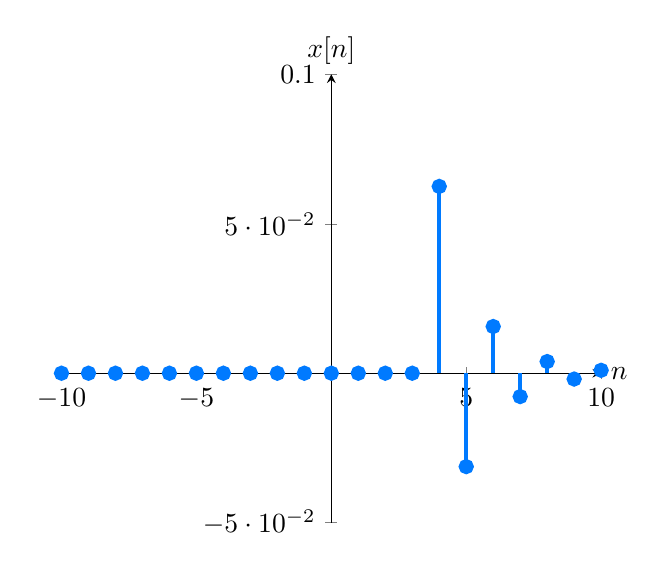
\begin{tikzpicture}
                \begin{axis}[
                    xmin= -10, xmax= 10,
                    ymin= -0.05, ymax = 0.1,
                    axis lines = middle,
                    xlabel={$n$}, ylabel={$x[n]$},
		  xlabel style={at={(axis cs:10,0)}, anchor=west},
        ylabel style={at={(axis cs:0,0.1)}, anchor=south},
                ]
                \addplot[lightblue, line width=1.5, ycomb, mark=*] coordinates {
                      (-10, 0.0)
(-9, -0.0)
(-8, 0.0)
(-7, -0.0)
(-6, 0.0)
(-5, -0.0)
(-4, 0.0)
(-3, -0.0)
(-2, 0.0)
(-1, -0.0)
(0, 0.0)
(1, -0.0)
(2, 0.0)
(3, -0.0)
(4, 0.0625)
(5, -0.03125)
(6, 0.015625)
(7, -0.0078125)
(8, 0.00390625)
(9, -0.001953125)
(10, 0.0009765625)
                    };
                \end{axis}
            \end{tikzpicture}\qquad
					\begin{tikzpicture}
                \begin{axis}[
                    xmin= -5, xmax= 5,
                    ymin= -0.1, ymax=16.1,
                    axis lines = middle,
                    xlabel={$n$}, ylabel={$h[n]$},
		  xlabel style={at={(axis cs:5,0)}, anchor=west},
        ylabel style={at={(axis cs:0,16.1)}, anchor=south},
                ]
                \addplot[lightblue, line width=1.5, ycomb, mark=*] coordinates {
(-5, 0.0009765625)
(-4, 0.00390625)
(-3, 0.015625)
(-2, 0.0625)
(-1, 0.25)
(0, 1.0)
(1, 4.0)
(2, 16.0)
(3, 0.0)
(4, 0.0)
(5, 0.0)
                    };
                \end{axis}
            \end{tikzpicture}
        \end{center}
        Por lo tanto, no hay traslape entre las señales, ya que $x[k]$ y  $h[n-k]$ no son simultáneamente no nulas para ningún  $n$. Esto implica que:  \[
            y[n]=0,\quad \forall n.
        \] 
    \item \db{$x[n]=2^nu[-n],\quad h[n]=u[n]$}

        Primero, analizamos los soportes de las señales:
        \begin{itemize}[label=\textbullet]
            \item $x[n]=2^nu[-n]$ está definida para  $n\le 0$.
            \item $h[n]=u[n]$ está definida para  $n\ge 0$.
        \end{itemize}
        \begin{center}
            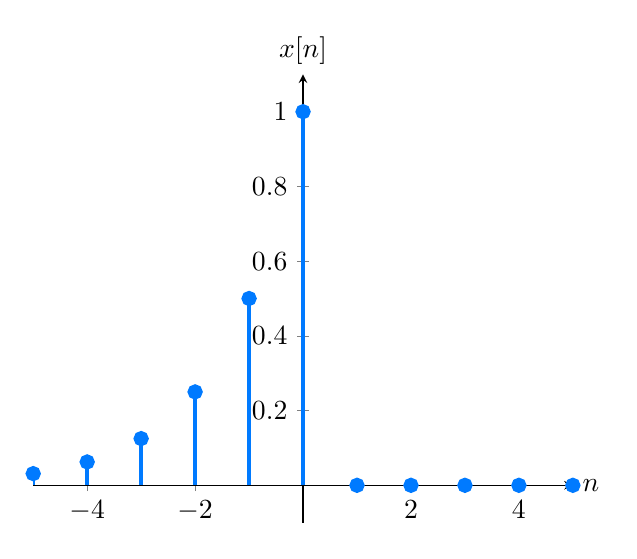
\begin{tikzpicture}
                \begin{axis}[
                    xmin= -5, xmax= 5,
                    ymin= -0.1, ymax = 1.1,
                    axis lines = middle,
                    xlabel={$n$}, ylabel={$x[n]$},
		  xlabel style={at={(axis cs:5,0)}, anchor=west},
        ylabel style={at={(axis cs:0,1.1)}, anchor=south},
                ]
                \addplot[lightblue, line width=1.5, ycomb, mark=*] coordinates {
(-5, 0.03125)
(-4, 0.0625)
(-3, 0.125)
(-2, 0.25)
(-1, 0.5)
(0, 1.0)
(1, 0.0)
(2, 0.0)
(3, 0.0)
(4, 0.0)
(5, 0.0)
                    };
                \end{axis}
            \end{tikzpicture}\qquad
				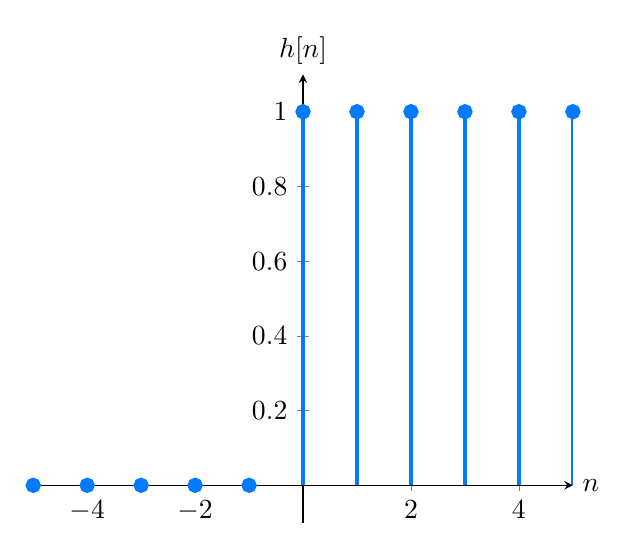
\begin{tikzpicture}
                \begin{axis}[
                    xmin= -5, xmax= 5,
                    ymin= -0.1, ymax = 1.1,
                    axis lines = middle,
                    xlabel={$n$}, ylabel={$h[n]$},
		  xlabel style={at={(axis cs:5,0)}, anchor=west},
        ylabel style={at={(axis cs:0,1.1)}, anchor=south},
                ]
                \addplot[lightblue, line width=1.5, ycomb, mark=*] coordinates {
(-5, 0.0)
(-4, 0.0)
(-3, 0.0)
(-2, 0.0)
(-1, 0.0)
(0, 1.0)
(1, 1.0)
(2, 1.0)
(3, 1.0)
(4, 1.0)
(5, 1.0)
                    };
                \end{axis}
            \end{tikzpicture}
        \end{center}
        La convolución es: \[
            y[n]=\sum_{k=-\infty}^{\infty} x[k]h[n-k]
        \] 

        Debido a los soportes de $x[k]$ y  $h[n-k]$, la suma solo es no nula cuando  $k\le 0$ y $n-k\ge 0$, es decir, $k\le 0$ y $k\ge n$. Esto implica que $n\le k\le 0$. Por lo tanto, la suma se reduce a: \[
            y[n]=\sum_{k=n}^{0} 2^k
        \] 
        Esta es una serie geométrica finita con razón $r=2$, y su suma es:  \[
        \sum_{k=n}^{0} 2^k=\dfrac{2^{0+1}-2^n}{1-2}=2\cdot (1-2^n)
        \] 
        Por lo tanto: \[
            y[n]=\begin{cases}
                2(1-2^n), & n\le 0\\
                0, & n>0
            \end{cases}
        \] 
\begin{center}
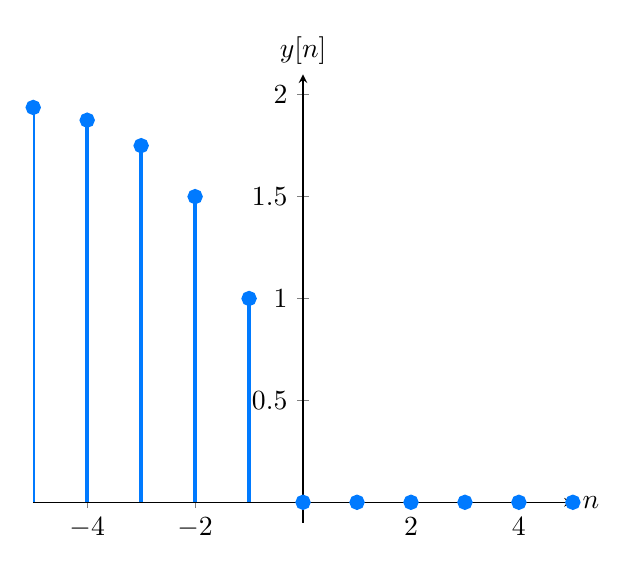
\begin{tikzpicture}
                \begin{axis}[
                    xmin= -5, xmax= 5,
                    ymin= -0.1, ymax = 2.1,
                    axis lines = middle,
                    xlabel={$n$}, ylabel={$y[n]$},
		  xlabel style={at={(axis cs:5,0)}, anchor=west},
        ylabel style={at={(axis cs:0,2.1)}, anchor=south},
                ]
                \addplot[lightblue, line width=1.5, ycomb, mark=*] coordinates {
(-5, 1.9375)
(-4, 1.875)
(-3, 1.75)
(-2, 1.5)
(-1, 1.0)
(0, 0.0)
(1, -0.0)
(2, -0.0)
(3, -0.0)
(4, -0.0)
(5, -0.0)
                    };
                \end{axis}
            \end{tikzpicture}
\end{center}
  \end{enumerate}
\item \lb{¿Cuál/es de las siguientes respuestas al impulso corresponden a sistemas LTI estables?} 
  \begin{enumerate}[label=\color{red}\textbf{\alph*)}]
    \item \db{$h(t)=e^{-(1-2j)t}u(t) $} 

        Primeros, descomponemos el exponente complejo: \[
        e^{-(1-2j)t}=e^{-t}e^{2jt}   
        \] 
        Aquí, $e^{-t} $ es una exponencial decreciente (para $t\ge 0$), y $e^{2jt} $ es una oscilación compleja de magnitud unitaria. Por lo tanto: \[
        |h(t)|=\left| e^{-t}e^{2jt}   \right| =|e^{-t} |=e^{-t},\quad t\ge 0. 
        \] 
        La integral de $|h(t)|$ es:  \[
            \int_{-\infty}^{\infty} |h(t)|\dt=\int_{0}^{\infty} e^{-t}\dt=[-e^{-t} ]_0^{\infty}=(0-(-1))=1.   
        \] 
        Por lo tanto, el sistema es \textbf{estable}. 
    \item \db{$h(t)=e^{-t}\cos(2t)u(t) $} 

        La función $\cos(2t)$ es una oscilación de magnitud unitaria, y $e^{-t} $ es una exponencial decreciente (para $t\ge 0$). Por lo tanto: \[
        |h(t)|=|e^{-t}\cos(2t) |\le e^{-t},\quad t\ge 0 .
        \] 
        La integral de $|h(t)|$ está acotada por la integral de  $e^{-t} $, que ya sabemos que converge: \[
        \int_{-\infty}^{\infty} |h(t)|\dt=\int_{0}^{\infty} |e^{-t}\cos(2t) |\dt\le \int_{0}^{\infty} e^{-t}\dt=1    
        \] 
        Por lo tanto, esta integral también converge, y el sistema es \textbf{estable}. 
  \end{enumerate}
\item \lb{¿Cuál/es de las siguientes respuestas al impulso corresponden a sistemas LTI estables?} 
  \begin{enumerate}[label=\color{red}\textbf{\alph*)}]
    \item \db{$h[n]=n\cos\left( \dfrac{\pi}{4} \right) $} 
    \item \db{$h[n]=3^nu[-n+10]$} 
  \end{enumerate}
\item \lb{Para las siguientes respuestas al impulso de sistemas LTI, determine si cada sistema es causal y/o estable, justificando la respuesta.}
  \begin{enumerate}[label=\color{red}\textbf{\alph*)}]
    \item \db{$h[n]=\left( \dfrac{1}{5} \right) ^nu[n]$} 

      \begin{itemize}[label=\textbullet]
        \item \textbf{Causalidad:} El término $u[n]$ asegura que  $h[n]=0$ para  $n<0$. Por lo tanto, el sistema es \lb{causal}.
        \item \textbf{Escalabilidad:} Para $n\ge 0,|h[n]|=\left( \dfrac{1}{5} \right) ^{n}$. La suma de esta serie geométrica es: \[
        \sum_{n=0}^{\infty} \left( \dfrac{1}{5} \right) ^n=\dfrac{1}{1-\frac{1}{5} }=\dfrac{5}{4}<\infty
        \] Por lo tanto, el sistema es \lb{estable} 
      \end{itemize}
    \item \db{$h[n]=0.8^nu[n+2]$} 
      \begin{itemize}[label=\textbullet]
        \item \textbf{Causalidad:} El término $u[n+2]$ implica que $h[n]\neq 0$ para $n\ge -2$. Como $h[n]\neq 0$ para $n<0$, el sistema  \lb{no es causal}.
        \item \textbf{Estabilidad:} Para $n\ge -2,|h[n]|=0.8^n$. Cambiando el índice de la suma $(m=n+2)$, tenemos:  \[
        \sum_{n=-2}^{\infty} 0.8^n=0.8^{-2}\sum_{m=0}^{\infty} 0.8^m=\dfrac{1}{0.8^2}\cdot \dfrac{1}{1-0.8}=\dfrac{1}{0.64}\cdot 5=7.8125<\infty
        \] 
        Por lo tanto, el sistema es \lb{estable}. 
      \end{itemize}
    \item  \db{$h[n]=\left( \dfrac{1}{2} \right) ^n u[-n]$} 

      \begin{itemize}[label=\textbullet]
        \item \textbf{Causalidad:} El término $u[-n]$ implica que $h[n]\neq 0$ solo para $n\le 0$. Esto significa que el sistema depende de valores futuros de la entrada, por lo que \lb{no es causal}.
        \item \textbf{Estabilidad:} Para $n\le 0,|h[n]|=\left( \dfrac{1}{2} \right) ^n=2^{-n}$. Cambiando el índice $(m=-n)$, tenemos:  \[
        \sum_{n=-\infty}^{0} 2^{-n}=\sum_{m=0}^{\infty} 2^m
        \] 
        Esta serie geométrica diverge, por lo que el sistema \lb{no es estable}. 
      \end{itemize}
    \item \db{$h[n]=5^nu[3-n]$} 
      \begin{itemize}[label=\textbullet]
        \item \textbf{Causalidad:} El término $u[3-n]$  implica que $h[n]\neq 0$ solo para $n\le 3$. Esto significa que el sistema depende de valores futuros de la entrada, por lo que \lb{no es causal}.
        \item \textbf{Estabilidad:} Para $n\le 3,|h[n]|=5^n$. Esta serie incluye términos crecientes (por ejemplo, $5^3$), por lo que no es absolutamente sumable. El sistema \lb{no es estable}. 
      \end{itemize}
    \item \db{$h[n]=\left( -\dfrac{1}{2} \right) ^nu[n]+1.01^nu[n-1]$} 
      \begin{itemize}[label=\textbullet]
        \item \textbf{Causalidad:} Ambos términos incluyen $u[n]$ o  $u[n-1]$, lo que asegura que $h[n]=0$ para $n<0$. Por lo tanto, el sistema es  \lb{causal}. 
        \item \textbf{Estabilidad:} EL primer término $\left( -\dfrac{1}{2} \right) ^{n}u[n]$ es absolutamente sumable, ya que: \[
        \sum_{n=0}^{\infty} \left| \left( -\dfrac{1}{2} \right) ^{n} \right| =\sum_{n=0}^{\infty} \left( \dfrac{1}{2} \right) ^n=2
        \] 
        Sin embargo, el segundo término $1.01^nu[n-1]$ crece exponencialmente y no es absolutamente sumable. Por lo tanto, el sistema  \lb{no es estable}.
      \end{itemize}
    \item \db{$h[n]=\left( -\dfrac{1}{2} \right) ^nu[n]+1.01^nu[1-n]$} 
      \begin{itemize}[label=\textbullet]
        \item \textbf{Causalidad:} El primer término $\left( -\dfrac{1}{2} \right) ^nu[n]$ es causal, pero el segundo término $1.01^nu[1-n]$ implica que  $h[n]\neq 0$ para  $n>1$. Por lo tanto, el sistema  \lb{no es causal}.
      \item \textbf{Estabilidad:} El primer término es aboslutamente sumable, pero el segundo término $1.01^nu[1-n]$ no lo es, ya que incluye términos crecientes. Por lo tanto, el sistema \lb{no es estable}.
      \end{itemize}
    \item \db{$h[n]=n\left( \dfrac{1}{3} \right) ^nu[n-1]$} 
      \begin{itemize}[label=\textbullet]
        \item \textbf{Causalidad:} El término $u[n-1]$  asegura que $h[n]=0$ para  $n<1$. Por lo tanto el sistema es  \lb{causal}.
        \item Para $n\ge 1,|h[n]|=n\left( \dfrac{1}{3} \right) ^n$ decrece exponencialmente, el factor $n$ hace que la serie no sea absolutamente sumable. Por ejemplo, usando el criterio de comparación, la serie diverge. Por lo tanto, el sistema  \lb{no es estable}. 
      \end{itemize}
  \end{enumerate}
\item \lb{Considere un sistema LTI que se encuentra incialmente en reposo y cuya entrada $x(t)$ y salida $y(t)$ se relacionan por la ecuación diferencial \[
\dfrac{\mathrm{d}}{\dt}y(t)+4y(t)=x(t)
\] } 
\begin{enumerate}[label=\color{red}\textbf{\alph*)}]
  \item \db{Obtenga la respuesta al impulso del sistema.}

		La ecuación diferencial que describe el sistema es:
		\[
		\dfrac{\mathrm{d}}{\dt}y(t)+4y(t)=x(t).
		\]
		Para encontrar la \textbf{respuesta al impulso} $h(t)$, consideramos la entrada $x(t)=\delta(t)$. En este caso, la ecuación difernecial se convierte en: \[\dfrac{\mathrm{d}}{\dt}y(t)+4h(t)=\delta(t).\]

\textbf{Resolviendo la ecuación diferencial}
\begin{itemize}[label=\textbullet]
\item \textbf{Ecuación homogénea:} Primero resolvemos la ecuación homogénea asociada $(x(t)=0)$: \[\dfrac{\mathrm{d}}{\dt}h_h(t)+4h_h(t)=0.\]
La solución general de esta ecuación es: \[h_h(t)=Ce^{-4t},\] donde $C$ es una constante que se determinará con las condiciones iniciales.
\item \textbf{Solución particular:} Dado que la entrada es un impulso $\delta(t)$, la solución particular se encuentra considerando la propiedad de causalidad del sistema LTI. La respuesta al impulso $h(t)$ debe ser cero para $t<0$. Además, integramos ambos lados de la ecuación diferencial en un intervalo infinitesimal alrededor de $t=0$ para determinar la discontinuidad en $h(t)$: \[\int_{-\epsilon}^\epsilon\left(\dfrac{\mathrm{d}}{\dt}h(t)+4h(t)\right)\dt=\int_{-\epsilon}^{\epsilon}\delta(t)\dt.\]
\end{itemize}
El primer término se evalúa como: \[
\int_{-\epsilon}^{\epsilon}\dfrac{\mathrm{d}}{\dt}h(t)\dt=h(\epsilon)-h(-\epsilon).  
\] 
Para un sistema causal, $h(t)=0$ para  $t<0$, por lo que  $h(-\epsilon)=0$. Esto implica: \[
h(\epsilon)-0+\int_{-\epsilon}^{\epsilon} 4h(t)\dt=1. 
\] 
En el límite $\epsilon\to 0$, el término $\int_{-\epsilon}^{\epsilon} 4h(t)\dt $ desaparece, y obtenemos: \[
h(0^+)=1.
\] 
\begin{itemize}[label=\textbullet]
    \item \textbf{Solución completa:} La solución completa es: \[
    h(t)=\begin{cases}
        e^{-4t}, & t\ge 0\\
        0, & t<0
    \end{cases}
    \]  
\end{itemize}
Por lo tanto, la \textbf{respuesta al impulso} del sistema es: \[
h(t)=e^{-4t}u(t), 
\]  donde $u(t)$ es la función escalón unitario.
  \item \db{Si $x(t)=e^{(-1+3j)t} u(t)$, calcule $y(t)$} 

      La salida de un sistema LTI se obitnee mediante la convolución de la entrada $x(t)$ con la respuesta al impulso  $h(t)$:  \[
      y(t)=x(t)\ast h(t)=\int_{-\infty}^{\infty} x(\tau)h(t-\tau)\mathrm{d}\tau. 
      \] 
      Sustituyendo $x(t)=e^{(-1+3j)t} u(t)$ y $h(t)=e^{-4t}u(t) $, tenemos: \[
      y(t)=\int_{-\infty}^{\infty} e^{(-1+3j)\tau}u(\tau)e^{-4(t-\tau)} u(t-\tau)\mathrm{d}\tau.
      \] 
      Debido a las funciones escalón $u(\tau)$ y  $u(t-\tau)$, los límites de integración se restringen a $0\le \tau\le t$. Por lo tanto: \[
      y(t)=\int_{0}^{t} e^{(-1+4j)\tau}e^{-4(t-\tau)}   \mathrm{d}\tau.
      \] 
      Simplificamos el exponente: \[
      e^{(-1+3j)\tau}e^{-4(t-\tau)}  =e^{-4t}e^{(3j-1+4)\tau}=e^{-4t}e^{(3j+3)\tau}.    
      \] 
      Entonces: \[
      y(t)=e^{-4t}\int_{0}^{t} e^{(3j+3)\tau}\mathrm{d}\tau.   
      \] 
      Resolvemos la integral: \[
      \int_{0}^{t} e^{(3j+3)\tau}\mathrm{d}\tau=\dfrac{1}{3j+3}\left[ e^{(3j+3)\tau}  \right] _0^t=\dfrac{1}{3j+3}\left( e^{(3j+3)t}-1  \right)   .
      \] 
      Por lo tanto: \[
      y(t)=e^{-4t}\cdot \dfrac{1}{3j+3}\left( e^{(3j+3)t}-1  \right)  =\dfrac{1}{3j+3}\left( e^{(-1+3j)t}-e^{-4t}   \right) .
      \] 
\end{enumerate}
\item \lb{Considere un sistema LTI que se encuentra inicialmente en reposo y cuya entrada  $x(t)$ y salida  $y(t)$ se relacionan por la ecuación diferencial  \[
\dfrac{\mathrm{d}}{\dt}y(t)+3y(t)=2x(t)
\] } 
\begin{enumerate}[label=\color{red}\textbf{\alph*)}]
  \item \db{Si $x(t)=\cos(2t)u(t)$, calcule $y(t)$.}

      La ecuación diferencia que describe el sistema es: \[
      \dfrac{\mathrm{d}}{\dt}y(t)+3y(t)=2x(t).
      \] 
      Dado que $x(t)=\cos(2t)u(t)$, la entrada es causal, y el sistema está inicialmente en resposo. Resolveremos esta ecuación diferencial para $y(t)$.
      \begin{center}
          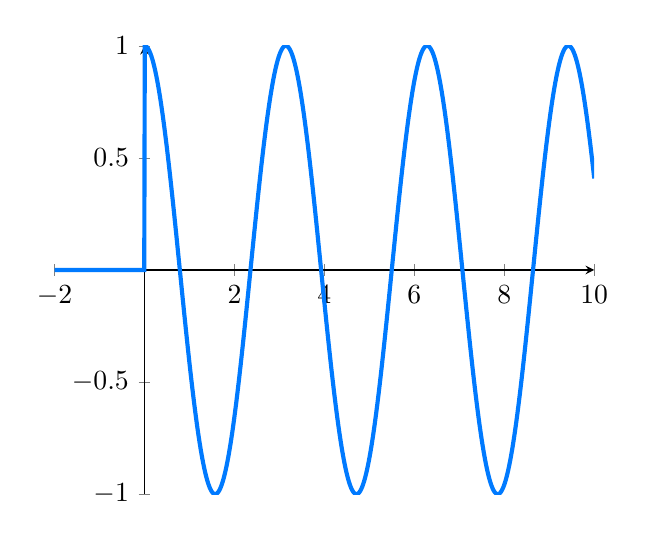
\begin{tikzpicture}
              \begin{axis}[
                  xmin= -2, xmax= 10,
                  ymin= -1, ymax = 1,
                  axis lines = middle,
              ]
                  \addplot[domain=-2:10, samples=1000, lightblue, line width=1.5]{x<0 ? 0 : cos(deg(2*x))};
              \end{axis}
          \end{tikzpicture}
      \end{center}
       \begin{enumerate}[label=Paso \arabic*:]
          \item Representación de la entrada

              La entrada $x(t)=\cos(2t)u(t)$ puede escribirse en términos de exponenciales complejas usando la identidad de Euler: \[
              \cos(2t)=\dfrac{e^{j2t}+e^{-j 2t}  }{2}.
              \] 
              Por lo tanto: \[
              x(t)=\dfrac{1}{2}\left( e^{j 2t}+e^{-j 2t}   \right) u(t).
              \] 
          \item Solución de la ecuación diferencial

              La solución general de la ecuación difernecial tiene dos componentes: \[
              y(t)=y_h(t)+y_p(t),
              \] donde $y_h(t)$ es la solución de la ecuación homogénea asociada  $(x(t)=0)$ y  $y_p(t)$ es una solución particular.
               \begin{enumerate}[label=\alph*)]
                  \item Solución homogénea

                      La ecuación homogénea es: \[
                      \dfrac{\mathrm{d}}{\dt}y_h(t)+3y_h(t).
                      \]
                      Resolviendo, obtenemos: \[
                      y(t)=Ce^{-3t} ,
                      \] donde $C$ es una constante que se determinará con las condiciones iniciales.
                  \item Solución particular

                      Para encontrar $y_p(t)$, asumimos una solución de la forma:  \[
                      y_p(t)=Ae^{j 2t}+Be^{-j 2t}.
                      \] 
                      Sustituyendo $y_p(t)$ en la ecuación diferencial:  \[
                      \dfrac{\mathrm{d}}{\dt}\left( Ae^{j 2t}+Be^{-j 2t}   \right) +3\left( Ae^{j 2t} +Be^{-j 2t}  \right) =2x(t).
                      \] 
                      Calculamos la derivada: \[
                      \dfrac{\mathrm{d}}{\dt}\left( Ae^{j 2t}+Be^{-j 2t}   \right) =j 2Ae^{j2t}-j2 Be^{-j2t}  .
                      \] 
                      Sustituyendo: \[
                          (j 2A+3A)e^{j2t} +(-j 2B+3B)e^{-j 2t}=2\cdot \dfrac{1}{2}\left( e^{j 2t}+e^{-j 2t}   \right)  .
                      \] 
                      Agrupando términos: \[
                          ((j 2+3)A)e^{j2t}+((-j 2+3)B)e^{-j 2t}=e^{j2t}+e^{-j 2t} .
                      \] 
                      Igualando coeficientes de $e^{j 2t} $ y $e^{-j 2t} $:
                      \begin{itemize}[label=\textbullet]
                          \item Para $e^{j 2t}:(j 2+3)A=1 $.
                          \item Para $e^{-j 2t}:(-j 2+3)B=1 $.
                      \end{itemize}
                      Resolviendo para $A$ y  $B$:  \[
                      A=\dfrac{1}{2j+3},\quad B=\dfrac{1}{-2j+3}.
                      \] 
                      Simplificamos $A$ y $B$ multiplicando numerador y denominador por el conjugado del denominador: \[
                      \begin{array}{c}
                          A=\dfrac{1}{2j+3}\cdot \dfrac{-2j+3}{-2j+3}=\dfrac{-2j+3}{(2j+3)(-2j+3)}=\dfrac{-2j+3}{13}\\
                          B=\dfrac{1}{-2j+3}\cdot \dfrac{2j+3}{2j+3}=\dfrac{2j+3}{(2j+3)(-2j+3)}=\dfrac{2j+3}{13}
                      \end{array}
                      \] 
                      Por lo tanto, la solución particular es: \[
                      y_p(t)=\dfrac{-2j+3}{13}e^{j 2t}+\dfrac{2j+3}{13}e^{-j 2t}.  
                      \] 
                      Usando la identidad de Euler para regresar a términos reales: \[
                      y_p(t)=\dfrac{3}{13}\cos(2t)+\dfrac{2}{13}\sin(2t).
                      \] 
                  \item Solución completa

                      La solución completa es:
                      \[
                      y(t)=y_h(t)+y_p(t)=Ce^{-3t}+\dfrac{3}{13}\cos(2t)+\dfrac{2}{13}\sin(2t). 
                      \] 
                      Dado que el sistema está inicialmente en reposo $(y(0)=0)$, sustituimos  $t=0$ para determinar  $C$:  \[
                      \begin{array}{c}
                          y(0)=C+\dfrac{3}{13}\cos(0)+\cancel{\dfrac{2}{13}\sin(0)} =0.\\
                          C+\dfrac{3}{13}=0\longrightarrow C=-\dfrac{3}{13}.
                      \end{array}
                      \] 
                      Por lo tanto, la solución final es: \[
                      y(t)=-\dfrac{3}{13}e^{-3t}+\dfrac{3}{13}\cos(2t)+\dfrac{2}{13}\sin(2t). 
                      \] 
              \end{enumerate}
      \end{enumerate}
  \item \db{Obtenga la respuesta al impulso del sistema.} 

      La respuesta al impulso $h(t)$ se obtiene resolviendo la ecuación diferencial con  $x(t)=\delta(t)$. La ecuación se convierte en:  \[
      \dfrac{\mathrm{d}}{\dt}h(t)+3h(t)=2\delta(t).
      \] 
      Integrando ambos lados en un intervalo infinitesimal alrededor de $t=0$, obtenemos:  \[
      \int_{-\epsilon}^{\epsilon} \dfrac{\mathrm{d}}{\dt}h(t)\dt+\int_{-\epsilon}^{\epsilon} 3h(t) \dt=\int_{-\epsilon}^{\epsilon} 2\delta(t)\dt.  
      \] 
      El primer término es $h(\epsilon)-h(-\epsilon)$, y dado que $h(t)=0$ para  $t< 0$, esto se reduce a $h(0^+)=2$. Por lo tanto, la solución es:  \[
      h(t)=Ce^{-3t}u(t). 
      \] 
      Usando $h(0^+)=2$, tenemos  $C=2$. Por lo tanto:  \[
      h(t)=2e^{-3t}u(t) .
      \] 
\end{enumerate}
\item \lb{Obtenga la respuesta al impulso, así como las propiedades de memoria, causalidad, estabilidad, invarianza en el tiempo y linealidad de los siguientes sistemas:}
  \begin{enumerate}[label=\color{red}\textbf{\alph*)}]
    \item \db{$y(t)=\int_{-\infty}^{t} x(\tau)\mathrm{d}\tau $} 

        \textbf{Respuesta al impulso}

        Para encontrar la respuesta al impulso $h(t)$, sustituimos  $x(t)=\delta(t)$:  \[
        y(t)=\int_{-\infty}^{t} \delta(\tau) \mathrm{d}\tau.
        \] 
        La integral de la delta de Dirac es la función escalón unitario $u(t)$. Por lo tanto:  \[
        h(t)=u(t).
        \] 
        \textbf{Propiedades}
        \begin{itemize}[label=\textbullet]
            \item \textbf{Memoria:} El sistema tiene memoria, ya que la salida en $t$ depende de los valores pasado de la entrada ($x(\tau)$ para $\tau\le t$).
            \item \textbf{Causalidad:} El sistema es causal, ya que la salida en $t$ depende únicamente de valores de la entrada para  $\tau\le t$.
            \item \textbf{Estabilidad:} El sistema no es estable. Por ejemplo, si $x(t)=1$ (una entrada acotada), la salida es  $y(t)=t$, que no está acotada.
            \item \textbf{Invarianza en el tiempo:} El sistema es invariante en el tiempo. Si desplazamos la entrada $x(t)$ por  $t_0$, la salida también se desplaza por $t_0$.
            \item \textbf{Linealidad:} El sistema es lineal, ya que satisface la superposición.
        \end{itemize}
    \item \db{$y(t)=\int_{-\infty}^{t} 2x(\tau-5)\mathrm{d}\tau $} 

        \textbf{Respuesta al impulso}

        Sustituyendo $x(t)=\delta(t)$:  \[
        y(t)=\int_{-\infty}^{t}  2\delta(\tau-5)\mathrm{d}\tau.
        \] 
        La delta de Dirac se activa en $\tau=5$, y la integral es cero para  $t<5$ y 2 para  $t\ge 5$. Por lo tanto: \[
        h(t)=2u(t-5).
        \] 
        \textbf{Propiedades}
        \begin{itemize}[label=\textbullet]
            \item \textbf{Memoria:} El sistema tiene memoria, ya que la salida depende de valores pasados de la entrada.
            \item \textbf{Causalidad:} El sistema no es causal, ya que la salida en $t$ depende de valores de la entrada en $\tau=t-5$, que puede ser un valor futuro si  $t<5$.
            \item \textbf{Estabilidad:} El sistema no es estable. Por ejemplo, si $x(t)=1$, la salida crece sin límite.
            \item \textbf{Invarianza en el tiempo:} El sistema es invariante en el tiempo. UN desplazamiento en la entrada produce un desplazamiento equivalente en la salida.
            \item \textbf{Linealidad:} El sistema es lineal, ya que satisface la superposición.
        \end{itemize}
    \item \db{$y(t)=\int_{-\infty}^{t} e^{-(t-\tau)} 3x(\tau-2)\mathrm{d}\tau $} 
       
        \textbf{Respuesta al impulso}

        Sustituyendo $x(t)=\delta(t)$:  \[
        y(t)=\int_{-\infty}^{t} e^{-(t-\tau)}3\delta(\tau-2)\mathrm{d}\tau.  
        \] 
        La delta de DIrac se activa en $\tau=2$, y la integral evalúa:  \[
        y(t)=3e^{-(t-2)} \text{ para }t\ge 2.
        \] 
        Por lo tanto: \[
        h(t)=3e^{-(t-2)} u(t-2).
        \] 
        \textbf{Propiedades}
        \begin{itemize}[label=\textbullet]
            \item \textbf{Memoria:} El sistema tiene memoria, ya que la salida depende de valores pasados de la entrada.
            \item \textbf{Causalidad:} El sistema no es causal, ya que la salida en $t$ depende de valores de la entrada  $\tau=t-2$, que puede ser un valor futuro si  $t<2$.
            \item \textbf{Estabilidad:} El sistema es estable. La respuesta al impulso $h(t)$ es absolutamente integrable, ya que:  \[
            \int_{-\infty}^{\infty} |h(t)|\dt=\int_{2}^{\infty} 3e^{-(t-2)}\dt=3.   
            \] 
            \item \textbf{Invarianza en el tiempo:} El sistema no es invariante en el tiempo debido al término $e^{-(t-\tau)} $, que depende explícitamente de $t$.
            \item \textbf{Linealidad:} El sistema es lineal, ya que satisface la superposición.
        \end{itemize}
    \item \db{$y(t)=\int_{t-3}^{t+2} e^{-(t+\tau)} x(\tau-2)\mathrm{d}\tau $} 
        
        \textbf{Respuesta al impulso}

        Sustituyendo $x(t)=\delta(t)$:  \[
        y(t)=\int_{t-3}^{t+2}e^{-(t+\tau)}\delta(\tau-2)\mathrm{d}\tau.
        \] 
        La delta de Dirac se activa en $\tau=2$, pero esto ocurre solo si  $t-3\le 2\le t+2$, es decir, si $t\in [1,5]$, En este intervalo, la integral evalúa: \[
            y(t)=e^{-(t+2)}\text{ para } t\in [1,5].
        \] 
        Fuera de este intervalo ($t<1$ o $t>5$), la integral es cero. Por lo tanto: \[
        h(t)=\begin{cases}
            e^{-(t+2)} , & 1\le t\le 5\\
            0, & \text{en otro caso}
        \end{cases}
        \] 
        \textbf{Propiedades}
        \begin{itemize}[label=\textbullet]
            \item \textbf{Memoria:} El sistema tiene memoria, ya que la salida depende de valores pasados de la entrada.
            \item \textbf{Causalidad:} El sistema no es causal, ya que la salida en $t$ depende de valores de la entrada en  $\tau-2$, que puede ser un valor futuro.
            \item \textbf{Estabilidad:} El sistema es estable. La respuesta al impulso $h(t)$ es absolutamente integrable, ya que está acotada en el intervalo $[1,5]$.
            \item \textbf{Invarianza en el tiempo:} El sistema no es invariante en el tiempo debido al término $e^{-(t+\tau)} $, que depende explícitamente de $t$.
            \item \textbf{Linealidad:} El sistema es lineal, ya que satisface la superposición.
        \end{itemize}
  \end{enumerate}
\item \lb{Un sistema discreto viene determinado por la relación entrada-salida \[
      y[n]=e^{j\frac{2\pi}{10} (n+2)}x[n-2]. 
\] Analice las propiedades de memoria, causalidad, estabilidad, invarianza en el tiempo y linealidad del sistema.}
\begin{enumerate}[label=\textbf{\arabic*)}]
    \item \textbf{Memoria}

        Un sistema tiene memoria si la salida en un instante $n$ depende de valores pasados o futuros de la entrada. Si la salida depende únicamente del valor actual de la entrada, el sistema es sin memoria.

        En este caso, la salida $y[n]$ depende de $x[n-2]$, que es un valor pasado de la entrada (desplazados dos unidades en el tiempo). Por lo tanto, \textbf{el sistema tiene memoria.}
    \item \textbf{Causalidad}

        Un sistema es causal si la salida en un instante $n$ depende únicamente de valores presentes o pasados de la entrada, es decir, no depende de valores futuros de la entrada.

        Aquí, $y[n]$ depende de $x[n-2]$, que es un valor pasado de la entrada. No hay dependencia de valores futuros de  $x[n]$. Por lo tanto,  \textbf{el sistema es causal.}
    \item \textbf{Estabilidad}

        Un sistema es estable si para toda entrada acotada $x[n]$, la salida $y[n]$ también es acotada. 

        La salida está dada por: \[
            y[n]=e^{j\frac{2\pi}{10} (n+2)}x[n-2]. 
        \] 
        El término $e^{j\frac{2\pi}{10} (n+2)} $ es una exponencial compleja de magnitud unitaria ($|e^{j\theta} |=1$ para cualquier $\theta$). Por lo tanto, si $x[n-2]$ es acotada,  $y[n]$ también será acotada. Esto implica que  \textbf{el sistema es estable}.
    \item \textbf{Invarianza en el tiempo} 

        Un sistema es invariante en el tiempo si un desplazamiento en la entrada produce un desplazamiento equivalente en la salida, sin cambiar la forma de la relación entrada-salida.

        Supongamos que desplazamos la entrada $x[n]$ por $k$ unidades, es decir, consideramos una nueva entrada $x_k[n]=x[n-k]$. La salida correspondiente sería:  \[
            y_k[n]=e^{j\frac{2\pi}{10} (n+2)}x_k[n-2]=e^{j\frac{2\pi}{10} (n+2)} x[n-k-2]. 
        \] 
        Comparando con la salida original $y[n]=e^{j\frac{2\pi}{10} (n+2)} x[n-2]$, vemos que el desplazamiento en la entrada introduce un cambio en el argumento de $x$, pero no se traduce en un simple desplazamiento de la salida. Esto significa que  \textbf{el sistema no es invariante en el tiempo.} 

    \item \textbf{Linealidad}

        Un sistema es lineal si satisface el principio de superposición, es decir, si para dos entradas $x_1[n]$ y $x_2[n]$ y sus respectivas salidas $y_1[n]$ y $y_2[n]$, se cumple que: \[
            a_1x_1[n]+a_2x_2[n]\longrightarrow a_1y_1[n]+a_2y_2[n].
        \] 
        En este caso, la relación entrada-salida es: \[
            y[n]=e^{j\frac{2\pi}{10} (n+2)} x[n-2].
        \] 
        Si la entrada es una combinación lineal $x[n]=a_1x_1[n]+a_2x_2[n]$, la salida será: \[
            y[n]=e^{j\frac{2\pi}{10} (n+2)}(a_1x_1[n-2]+a_2x_2[n-2])=a_1e^{j\frac{2\pi}{10} (n+2)} x_1[n-2]+a_2e^{j\frac{2\pi}{10} (n+2)}x_2[n-2]  .
        \] 
        Esto corresponde a $a_1y_1[n]+a_2y_2[n]$, lo que demuestra que \textbf{el sistema es lineal.} 
\end{enumerate}
\item \lb{Considere la señal $x[n]=\bigwedge\left( \dfrac{n}{4} \right) +\prod\left( \dfrac{n-2}{5} \right) $. Obtenga y represente la parte par e impar de esta señal. Calcule la energía y potencia de $x[n]$, indicando si se trata de una señal defindia en energía o en potencia.}

    \begin{enumerate}[label=\textbf{\arabic*)}]
        \item \textbf{Parte par e impar de la señal}

            La parte par $(x_e[n])$ y la parte impar  $(x_o[n])$ de una señal  $x[n]$ se definen como:  \[
                x_e[n]=\dfrac{x[n]+x[-n]}{2},\quad x_o=\dfrac{x[n]-x[-n]}{2}.
            \] 
            \begin{enumerate}[label=\alph*)]
                \item Cálculo de $x[-n]$

                    La señal invertida en el tiempo es:  \[
                        x[-n]=\bigwedge\left( \dfrac{-n}{4} \right) +\prod\left( \dfrac{-n-2}{5} \right) .
                    \] 
                \item Parte par $(x_e[n])$
 
                    Sustituyendo en la fórmula de la parte par: \[
                        x_e[n]=\dfrac{\bigwedge\left( \frac{n}{4}  \right) +\prod\left( \frac{n-2}{5}  \right) +\bigwedge\left( \frac{-n}{4}  \right) +\prod\left( \frac{-n-2}{5}  \right) }{2}.
                    \] 
                \item Parte impar $(x_o[n])$

                    Sustituyendo en la fórmula de la parte impar:  \[
                        x_o[n]=\dfrac{\bigwedge\left( \frac{n}{4}  \right) +\prod\left( \frac{n-2}{5}  \right) -\bigwedge\left( \frac{-n}{4}  \right) -\prod\left( \frac{-n-2}{5}  \right) }{2}.
                    \] 
            \end{enumerate}
            Para obtener las expresiones explícitas de $x_e[n]$ y  $x_o[n]$, se necesita evaluar las propiedades de simetría de las funciones  $\bigwedge$ y  $\prod$:
             \begin{itemize}[label=\textbullet]
                \item La función triangular $\bigwedge(x)$ es  \textbf{par}, es decir, $\bigwedge(-x)=\bigwedge(x)$ .
                \item La función rectangular $\prod(x)$ es  \textbf{par}, es decir, $\prod\left( -x \right) =\prod(x)$ .
            \end{itemize}
            Por lo tanto:
            \begin{itemize}[label=\textbullet]
                \item $\bigwedge\left( \dfrac{-n}{4} \right) =\bigwedge\left( \dfrac{n}{4} \right) $.
                \item $\prod\left( \dfrac{-n-2}{5} \right) =\prod\left( \dfrac{n+2}{5} \right) $.
            \end{itemize}
            Sustituyendo estas propiedades: \[
            \begin{array}{c}
                x_e[n]=\dfrac{\bigwedge\left( \frac{n}{4} \right)+\prod\left( \frac{n-2}{5}  \right) + \bigwedge\left( \frac{n}{4}  \right) +\prod\left( \frac{n+2}{5}  \right) }{2}=\bigwedge\left( \dfrac{n}{4} \right) +\dfrac{\prod\left( \frac{n-2}{5}  \right) +\prod\left( \frac{n+2}{5}  \right) }{2}. \\
                x_o[n]=\dfrac{\bigwedge\left( \frac{n}{4}  \right) +\prod\left( \frac{n-2}{5}  \right) -\bigwedge\left( \frac{n}{4}  \right) -\prod\left( \frac{n+2}{5}  \right) }{2}=\dfrac{\prod\left( \frac{n-2}{5}  \right) -\prod\left( \frac{n+2}{5}  \right) }{2}.
            \end{array}
            \] 
        \item \textbf{Cálculo de energía y potencia}

            La energía de una señal $x[n]$ se define como: \[
                E_x=\sum_{n=-\infty}^{\infty} |x[n]|^2.
            \] 
            La potencia de una señal $x[n]$ se define como:  \[
                P_x=\lim_{N \to \infty} \dfrac{1}{2N+1}\sum_{n=-N}^{N} |x[n]|^2.
            \] 
            \begin{enumerate}[label=\alph*)]
                \item Naturaleza de la señal $x[n]$

                    La señal  $x[n]$ está compuesta por una función triangular $\left( \bigwedge \right) $ y una función rectangular $\left( \prod \right) $, ambas de soporte finito. Esto significa que $x[n]$ es no nula solo en el intervalo finito de  $n$. Por lo tanto, la suma de  $|x[n]|^2$ será finita, y la energía será finita. Además, dado que la señal no es periódica y tiene soporte finito, su potencia será cero.
                \item Cálculo de la energía

                    Para calcular la energía, evaluamos: \[
                    E_x=\sum_{n=-\infty}^{\infty} \left| \bigwedge\left( \dfrac{n}{4} \right) +\prod\left( \dfrac{n-2}{5} \right)  \right| ^2.
                    \] 
                    Dado que $\bigwedge(x)$ y  $\prod(x)$ tienen soporte finito, la suma se produce a un intervalo finitp de  $n$. La energía se puede calcular explícitamente evaluando  $x[n]$ en los puntos donde no es cero.
                \item Potencia

                    La potencia será:  \[
                        P_x=\lim_{N \to \infty} \dfrac{1}{2N+1}\sum_{n=-N}^{N} |x[n]|^2.
                    \] 
                    Dado que $x[n]$ tiene soporte finito, la suma $\sum_{n=-N}^{N} |x[n]|^2$ no crece con $N$, y al dividir entre $2N+1$, el resultado tiende a cero. Por lo tanto, la potencia es:  \[
                    P_x=0.
                    \] 
            \end{enumerate}
            Por lo tanto, \textbf{la señal está definida en energía.} 
    \end{enumerate}

\item \lb{Calcule la convolución de las señales \[
      x_1[n]=(n-6)\prod\left( \dfrac{n-6}{13} \right) \qquad x_2[n]=\prod\left( \dfrac{-n-3}{5} \right) 
\] \underline{Nota:} la suma de una progresión aritmética $a_{n_i}, a_{n_i+1},\dots,a_{n_f}$, con $a_{n_i+1}=a_{n_i}+d,a_{n_i+2}=a_{n_i}+2d,\dots$ es \[
\sum_{k=n_i}^{n_f} a_k=\dfrac{(n_f-n_i+1)(a_{n_i}+a_{n_f})}{2}.
\] }

\begin{enumerate}[label=\textbf{\arabic*)}]
    \item \textbf{Soporte de las señales}
        \begin{enumerate}[label=\alph*)]
            \item Soporte de $x_1[n]$

                La función rectangular $\prod\left( \dfrac{n-6}{13} \right) $ es no nula solo cuando: \[
                \left| \dfrac{n-6}{13} \right| \le \dfrac{1}{2}\longrightarrow -\dfrac{13}{2}\le n-6\le \dfrac{13}{2}\longrightarrow -\dfrac{1}{2}\le n\le \dfrac{25}{2}.
                \] 
                Dado que $n$ es un número entero, el soporte de $x_1[n]$ es: \[
                    n\in \{0,1,2,\dots,12\} .
                \] 
            \item Soporte de $x_2[n]$

                La función rectangular $\prod\left( \dfrac{-n-3}{5} \right) $ es no nula solo cuando: \[
                \left| \dfrac{-n-3}{5} \right| \le \dfrac{1}{2}\longrightarrow -\dfrac{5}{2}\le -n-3\le \dfrac{5}{2}\longrightarrow -\dfrac{1}{2}\le -n\le \dfrac{11}{2}\longrightarrow -\dfrac{11}{2}\le n\le \dfrac{1}{2}.
                \] 
                Dado que $n$ es un número entero, el soporte de $x_2[n]$ es: \[
                n\in \{-5,-4,-3,-2,-2,-1,0\}. 
                \] 
        \end{enumerate}
    \item \textbf{Soporte de la convolución}

        El soporte de la convolución $y[n]=(x_1\ast x_2)[n]$ es la suma de los soportes de $x_1[n]$ y $x_2[n]$. Como el soporte de $x_1[n]$ es $\{0,1,\dots,12\} $ y el soporte de $x_2[n]$ es $\{-5,-4,\dots,0\} $, $y[n]$ será no nula en  $n\in \{-5,-4,\dots,12\} $.

    \item \textbf{Expresión de la convolución}

        La convolución se calcula como: \[
            y[n]=\sum_{k=-\infty}^{\infty} x_1[k]x_2[n-k].
        \] 
        Dado que $x_1[k]$ y $x_2[n-k]$ son no nulas solo en sus respectivos soportes, la suma se reduce a los valores de $k$ donde ambos términos son no nulos. Esto ocurre cuando: \[
        k\in \{0,1,\dots,12\} ,\quad n-k\in \{-5,-4,\dots,0\} .
        \] 
        Para que $n-k\in \{-5,-4,\dots,0\} $, se tiene: \[
        -5\le n-k\le 0\longrightarrow n\le k+5\text{ y }k\le n.
        \] 
        Por lo tanto, los valores de $k$ están restringidos por: \[
        \max(0,n-5)\le k\le \min(12,n).
        \] 
        La convolución se convierte en: \[
            y[n]=\sum_{k=\max(0,n-5)}^{\min(12,n)} (k-6)\prod\left( \dfrac{k-6}{13} \right) \prod\left( \dfrac{-(n-k)-3}{5} \right) .
        \] 
    \item \textbf{Evaluación de los productos}
        \begin{enumerate}[label=\alph*)]
            \item Propiedades de $\prod(x)$

                La función rectangular  $\prod(x)$ es igual a 1 cuando  $|x|\le \dfrac{1}{2}$ y 0 en otro caso. Por lo tanto:
                \begin{itemize}[label=\textbullet]
                    \item $\prod\left( \dfrac{k-6}{13} \right) $ si $k\in \{0,1,\dots,12\} $, y $0$ en otro caso.
                    \item  $\prod\left( \dfrac{-(n-k)-3}{5} \right) =1$ si $n-k\in \{-5,-4,\dots,0\} $, y 0 en otro caso.
                \end{itemize}
                Esto asegura que la suma realiza únicamente en el intervalo $k\in [\max(0,n-5),\min(12,n)]$.
        \end{enumerate}
    \item \textbf{Suma de una progresión aritmética} 

        Dentro del intervalo válido para $k$, el término $k-6$ forma una progresión aritmética con diferencia $d=1$. La suma de una progresión aritmética  $a_k=k-6$ desde  $k=k_{\min}$ hasta $k_{\max}$ es: \[
        \sum_{k=k_{\min}}^{k_{\max}}(k-6)=\dfrac{(k_{\max}-k_{\min}+1)((k_{\min})-6)+(k_{\max}-6)}{2}. 
        \] 
        Aquí: \[
        k_{\min}=max(0,n-5),\quad k_{\max}=\min(12,n).
        \] 
\end{enumerate}
\item \lb{Se pretende procesar la señal $x(t)$ de la figura con un sistema LTI cuya respuesta al impulso es  \[
h(t)=t\prod\left( \dfrac{2t-4}{8} \right) -2\delta(t+12)
\] } 
\begin{center}
\begin{tikzpicture}
    \begin{axis}[
        axis lines=middle,
        xmin=-10, xmax=10,
        ymin=-2.2, ymax=2.2,
        xlabel={$t$}, ylabel={$x(t)$},
        samples=500,
        xtick={-8,-6,-4,-2,0,2,4,6,8},
        ytick={-2,-1,0,1,2},
		  width=15cm, height=6cm,
		  xlabel style={at={(axis cs:10,0)}, anchor=west},
        ylabel style={at={(axis cs:0,2.2)}, anchor=south},
    ]

    \addplot[lightblue, ultra thick] coordinates {
        (-10,0) (0,0) (0,2) (4,2) (4,-2) (8,-2) (8,0) (9,0)
    };
    \end{axis}
\end{tikzpicture}
\end{center}
\begin{enumerate}[label=\color{red}\textbf{\alph*)}]
    \item \db{Obtenga la salida del sistema $y(t)$.} 

        La salida $y(t)$ de un sistema LTI se obtiene mediante la convolución de la entrada  $x(t)$ con la respuesta al impulso $h(t)$: \[
        y(t)=x(t)\ast h(t)=\int_{-\infty}^{\infty} x(\tau)h(t-\tau)\mathrm{d}\tau. 
        \] 
        \textbf{Respuestal al impulso $h(t)$:} \[
        h(t)=t\prod\left( \dfrac{2t-4}{8} \right) -2\delta(t+12).
        \]  
        \begin{itemize}[label=\textbullet]
            \item El término $t\prod\left( \dfrac{2t-4}{8} \right) $ es un pulso triangular centrado en $t=2$ con un ancho de 4 (no nulo para $t\in [0,4]$).
            \item El término $-2\delta(t+12)$ es una función delta de Dirac escalada en  $t=-12$.
        \end{itemize}   
        \textbf{Señal de entrada $x(t)$:}

        De la figura, $x(t)$ es un pulso rectangular definido como:  \[
        x(t)=\begin{cases}
            2, & 0\le t<4\\
            -2, & 4\le t<8\\
            0, & \text{en otro caso}
        \end{cases}
        \] 
        \begin{enumerate}[label=Paso \arabic*:]
            \item Descomposición de la convolución

                La convolución se puede dividir en dos términos debido a la estructura de $h(t)$:
                 \[
                y(t)=\left( x(t)\ast t\prod\left( \dfrac{2t-4}{8} \right)  \right) -2(x(t)\ast\delta(t+12)).
                \] 
                \begin{enumerate}[label=\alph*)]
                    \item Convolución con $\delta(t+12)$:

                        La convolución con la delta desplaza la entrada  $x(t)$ por $-12$:  \[
                        x(t)\ast \delta(t+12)=x(t+12).
                        \] 
                        Como $x(t)$ es no nula solo para $t\in [0,8],x(t+12)$ será no nula para $t\in [-12,4]$. Por lo tanto: \[
                        -2(x(t)\ast\delta(t+12))=\begin{cases}
                            -4, & -12\le t<-8\\
                            4, & -8\le t<-4\\
                            0, & \text{en otro caso}
                        \end{cases}
                        \] 
                    \item Convolución con $t\prod\left( \dfrac{2t-4}{8} \right) $ :

                        El término $t\prod\left( \dfrac{2t-4}{8} \right) $ es un pulso triangular centrado en $t=2$ con un ancho de 4 (no nulo para $t\in [0,4]$). La convolución iimplica entregar la superposición de $x(\tau)$ y el pulso triangular desplazado $t\prod\left( \dfrac{2(t-\tau)-4}{8} \right) $.
                \end{enumerate}
            \item Soportes de las señales

                \textbf{Soporte de $x(t)$:}

                La señal $x(t)$ es no nula para  $t\in [0,8]$.

                \textbf{Soporte de $t\prod\left( \dfrac{3t-4}{8} \right) $ :} 

                El pulso tringular es no nulo para $t\in [0,4]$.

                \textbf{Soporte de la convolución:}

                El soporte de la convolución es la suma de los soporte de $x(t)$ y $t\prod\left( \dfrac{2t-4}{8} \right) $, es decir: \[
                    [0,8]+[0,4]=[0,12].
                \] 
                Por lo tanto, $y(t)$ será no nula para $t\in [0,12]$.
            \item Evaluación de la convolución

                La convolución se evalúa como: \[
                y(t)=\int_{-\infty}^{\infty} x(\tau)\cdot (t-\tau)\prod\left( \dfrac{2(t-\tau)-4}{8} \right) \mathrm{d}\tau. 
                \] 
                \begin{enumerate}[label=\alph*)]
                    \item Intervalos de integración:

                        La integral se evalúa en los intervalos donde $x(\tau)$ y $(t-\tau)\prod\left( \dfrac{2(t-\tau)-4}{8} \right) $ se superponen. Esto depende de $t$:
                         \begin{itemize}[label=\textbullet]
                            \item Para $0\le t<4$, el pulso triangular está completamente dentro del soporte de $x(t)$.
                            \item Para  $4\le t<8$, el pulso triangular se superpone parcialmente con $x(t)$.
                            \item Para  $8\le t<12$, le pulso traingular se superpone con la segunda parte de $x(t)$.
                        \end{itemize}
                    \item Evaluación en cada intervalo:
                        \begin{itemize}[label=\textbullet]
                            \item Para $0\le t<4$:

                                En este intervalo, el pulso triangular está completamente dentro del soporte de $x(t)$. La integral es:  \[
                                y(t)=\int_{0}^{t} 2(t-\tau)\mathrm{d}\tau=2 \int_{0}^{t} (t-\tau)\mathrm{d}\tau=2\left[ t \tau-\dfrac{\tau^2}{2} \right] _0^t=2\left[ t^2-\dfrac{t^2}{2} \right] =t^2.  
                                \] 
                            \item Para $4\le t<8$:

                                En este intervalo, el pulso triangular se superpone parcialmente con $x(t)$. La integral se divide en dos partes: \[
                                y(t)=\int_{0}^{4} 2(t-\tau)\mathrm{d}\tau+\int_{4}^{t} -2(t-\tau)\mathrm{d}\tau.  
                                \] 
                                Resolviendo cada término:
                                \begin{itemize}[label=\textbullet]
                                    \item Para $\int_{0}^{4} 2(t-\tau)\mathrm{d}\tau $: \[
                                            \int_{0}^{4} 2(t-\tau)\mathrm{d}\tau=2\left[ t \tau-\dfrac{\tau^2}{2} \right] _0^4=2[4t-8]=8t-16. 
                                    \] 
                                \item Para $\int_{4}^{t} -2(t-\tau)\mathrm{d}\tau $ : \[
                                \int_{4}^{t} -2(t-\tau)\mathrm{d}\tau=-2\left[ t \tau-\dfrac{\tau^2}{2} \right] _4^t=-2\left[ t^2-\dfrac{t^2}{2} -(4r-8)\right]  =-2\left[ \dfrac{t^2}{2}-4t+8 \right] =-t^2+8-16
                                \] 
                                \end{itemize}
                                    Sumando ambos términos: \[
                                    y(t)=(8t-16)+(-t^2+8t-16)=-t^2+16t-32
                                    \] 
                                \item Para $8\le t<12$:

                                    En este intervalo, el pulso triangular se superpone con la segunda parte de $x(t)$. La integral es:  \[
                                        \begin{aligned}
                                    y(t)&= \int_{t-4}^{8} -2(t-\tau)\mathrm{d}\tau=-2 \int_{t-4}^{7} (t-\tau)\mathrm{d}\tau=-2\left[ t \tau-\dfrac{\tau^2}{2} \right] _{t-4}^{8}\\
                                        & =-2\left[ 8t-32-\left( t^2-4t-\dfrac{t^2-8t+16}{2} \right)  \right]  \\
                                        &= -2\left[ 16t-64-(2t^2-8t-t^2+8t-16) \right]=-2\left[ -t^2+16t-48 \right]   \\
                                        &= 2t^2-32t+96 \\
                                        \end{aligned}
                                    \] 
                        \end{itemize}
                \end{enumerate}
                La salida $y(t)$ es una función por tramos definida como:  \[
                y(t)=\begin{cases}
                    t^2, & 0\le t<4\\
                    -t^2+16t-32, & 4\le t<8\\
                    2t^2-32t+96, & 8\le t<12
                \end{cases}
                \] 
                \begin{center}
                    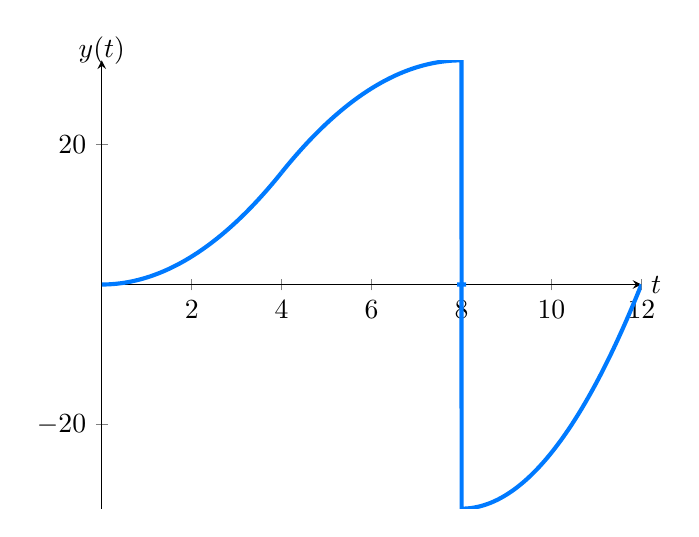
\begin{tikzpicture}
                        \begin{axis}[
                            xlabel={$t$}, ylabel={$y(t)$},
                            axis lines = middle,
                            xlabel style={at={(axis cs:12,0)}, anchor=west},
                            ylabel style={at={(axis cs:0,30)}, anchor=south},
                        ]
                            \addplot[domain=0:4, samples=1000, lightblue, line width=1.5] {x^2};
                            \addplot[domain=4:8.1, samples=1000, lightblue, line width=1.5] {x>8 ? 0 : -x^2+16*x-32};
                            \addplot[domain=7.9:12, samples=1000, lightblue, line width=1.5] {x<8 ? 0 : 2*x^2-32*x+96};
                        \end{axis}
                    \end{tikzpicture}
                \end{center}
        \end{enumerate}
    \item \db{Indique razonadamente si este sistema posee las propiedades de memoria, causalidad y estabilidad.}

        \begin{itemize}[label=\textbullet]
            \item \textbf{Memoria}
                \begin{itemize}[label=\textbullet]
                    \item El sistema tiene memoria porque la respuesta al impulso $h(t)$ depende de $t$ y no solo del valor actual de la entrada.
                \end{itemize}
            \item \textbf{Causalidad:}
                \begin{itemize}[label=\textbullet]
                    \item El sistema \textbf{no es causal} porque la respuesta al impulso $h(t)$ incluye un término $-2\delta(t+12)$, que depende de valores futuros del entrada (por ejemplo, $t=-12$)
                \end{itemize}
            \item \textbf{Estabilidad:}
                \begin{itemize}[label=\textbullet]
                    \item El sistema es \textbf{estable} porque la respuesta al impulso $h(t)$ es absolutamente integrable: \[
                    \int_{-\infty}^{\infty} |h(t)|\dt<\infty. 
                    \] 
                \end{itemize}
        \end{itemize}
    \item \db{Calcule la energía total y la potencia media de $x(t)$, e indique si está definida en energía o en potencia.}

        \begin{itemize}[label=\textbullet]
            \item \textbf{Energía:}

                La energía de $x(t)$ se define como:  \[
                E_x=\int_{-\infty}^{\infty} |x(t)|^2\dt. 
                \] 
                Como $x(t)$ es constante por partes: \[
                    E_x=\int_{0}^{4} |2|^2\dt+\int_{4}^{8} |-2|^2\dt=\int_{0}^{4} 4\dt+\int_{4}^{8} 4\dt=4[t]_{0}^4+4[t]_4^8 =16+16=32.
                \] 
            \item \textbf{Potencia:}

                La potencia promedio de $x(t)$ es:  \[
                P_x=\lim_{T \to \infty} \dfrac{1}{2T}\int_{-T}^{T} |x(t)|^2\dt=\lim_{T \to \infty} \dfrac{E_x}{2T}=\dfrac{32}{\infty}=0. 
                \] 
        \end{itemize}
        $x(t)$ es una  \textbf{señal definida en energía} porque tiene energía infinita y potencia nula. 
    \item \db{A partir del resultado del apartado (a), y utilizando únicamente propiedades de la convolución, obtenga la salida del sistema frente a la entrada \[
    z(t)=8\bigwedge\left( \dfrac{t-4}{4} \right) 
    \] } 
    La función triangular $\bigwedge\left( \dfrac{t-4}{4} \right) $ es una versión escalada y desplazada de un pulso triangular. Usando las propiedades de la convolución.
    \begin{itemize}[label=\textbullet]
        \item \textbf{Propiedades de escalamiento:} 

            Si $x(t)\ast h(t)=y(t)$, entonces  $[a\cdot x(t)]\ast h(t)=a\cdot y(t)$. Aquí, $z(t)=8\cdot \bigwedge\left( \dfrac{t-4}{4} \right) $, por lo que la salida se escala por 8.
        \item \textbf{Propiedad de desplazamiento:}

            Si $x(t)\ast h(t)=y(t)$, entonces  $x(t-t_0)\ast h(t)=y(t-t_0)$. El pulso triangular $\bigwedge\left( \dfrac{t-4}{4} \right) $ está desplazado en 4. Por lo tanto, la salida también se desplaza.
    \end{itemize}
    Usando estas propiedades, la salida para $z(t)$ es:  \[
    y_z(t)=8\cdot y(t-4),
    \] donde $y(t)$ es el resultado de la parte (a).





\end{enumerate}

\item \lb{Se pretende procesar la señal $x[n]=\sin\left( \dfrac{\pi}{4}n \right) u[n]$ con un sistema LTI cuya respuesta al impulso es $h[n]=\sin\left( \dfrac{\pi}{4}n \right) u[n+2]$.}

    \begin{enumerate}[label=\color{red}\textbf{\alph*)}]

        \item \db{Represente en detalle $x[n]$ y  $h[n]$.}

            \begin{center}
                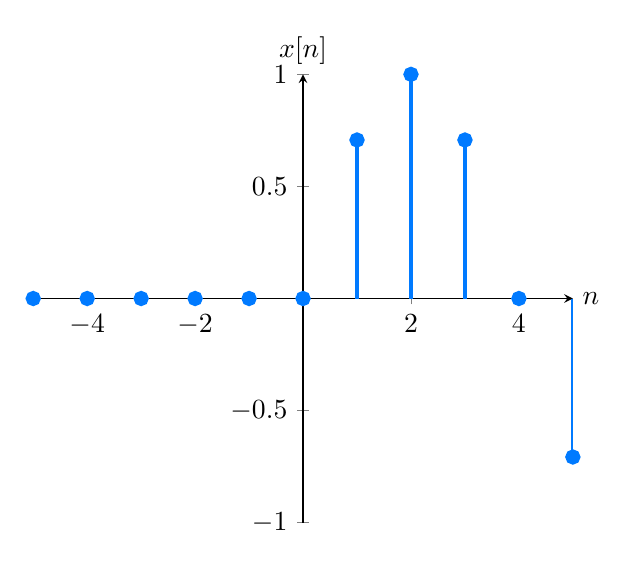
\begin{tikzpicture}
                    \begin{axis}[
                        xmin= -5, xmax= 5,
                        ymin= -1, ymax = 1,
                        axis lines = middle,
                        xlabel={$n$}, ylabel={$x[n]$},
                        xlabel style={at={(axis cs:5,0)}, anchor=west},
                        ylabel style={at={(axis cs:0,1)}, anchor=south},
                    ]
                    \addplot[lightblue, line width=1.5, ycomb, mark=*] coordinates {
                            (-5, 0.0)
                             (-4, -0.0)
                              (-3, -0.0)
                               (-2, -0.0)
                                (-1, -0.0)
                                 (0, 0.0)
                                  (1, 0.7071067811865475)
                                   (2, 1.0)
                                    (3, 0.7071067811865476)
                                     (4, 1.2246467991473532e-16)
                                      (5, -0.7071067811865475)
                        };
                    \end{axis}
                \end{tikzpicture}\qquad
                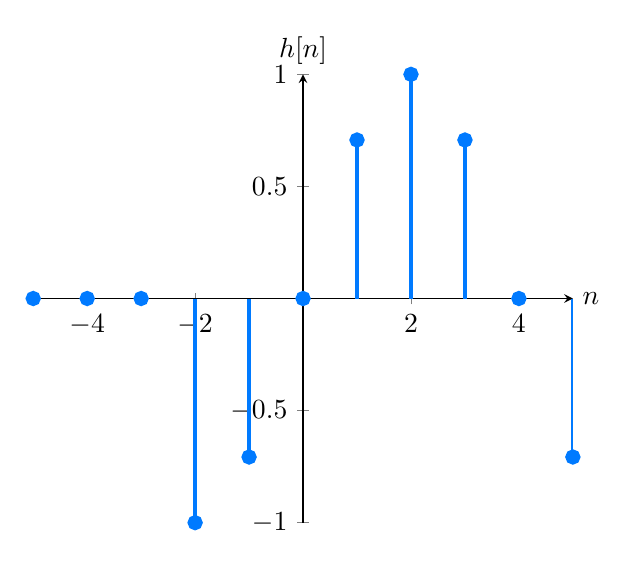
\begin{tikzpicture}
                    \begin{axis}[
                        xmin= -5, xmax= 5,
                        axis lines = middle,
                        xlabel={$n$}, ylabel={$h[n]$},
                        xlabel style={at={(axis cs:5,0)}, anchor=west},
                        ylabel style={at={(axis cs:0,1)}, anchor=south},
                    ]
                    \addplot[ycomb, mark=*, lightblue, line width=1.5] coordinates {
                            (-5, 0.0)
                             (-4, -0.0)
                              (-3, -0.0)
                               (-2, -1.0)
                                (-1, -0.7071067811865475)
                                 (0, 0.0)
                                  (1, 0.7071067811865475)
                                   (2, 1.0)
                                    (3, 0.7071067811865476)
                                     (4, 1.2246467991473532e-16)
                                      (5, -0.7071067811865475)
                        };
                    \end{axis}
                \end{tikzpicture}
            \end{center}
        \item \db{Indique razonadamente si este sistema definido por $h[n]$ posee las propiedades de memoria, causalidad y estabilidad.}

            El sistema está definido por su respuesta al impulso $h[n]$. Analizamos las propiedades:
             \begin{itemize}[label=\textbullet]
                \item \textbf{Memoria:}
                    \begin{itemize}[label=\textbullet]
                        \item Un sistema tiene memoria si su salida depende de valores pasados o futuros de la entrada.
                        \item En este caso, $h[n]$ depende de  $n$, lo que implica que el sistema tiene memoria.
                    \end{itemize}
                \item \textbf{Causalidad:}
                    \begin{itemize}[label=\textbullet]
                        \item Un sistema es causal si su salida en un instante $n$ depende solo de valores presentes o pasados de la entrada.
                        \item Como $h[n]$ es no nula para $n\ge -2$, el sistema \textbf{no es causal}, ya que depende de valores futuros de la entrada (por ejemplo, $n=-2$). 
                    \end{itemize}
                \item \textbf{Estabilidad:}
                    \begin{itemize}[label=\textbullet]
                        \item Un sistema es estable si su respuesta al impulso $h[n]$ es absolutamente sumable, es decir:  \[
                                \sum_{n=-\infty}^{\infty} |h[n]|<\infty.
                        \] 
                    \item En este caso, $h[n]=\sin\left( \dfrac{\pi}{4}n \right) u[n+2]$ no es absolutamente sumable porque $\sin\left( \dfrac{\pi}{4}n \right) $ no decrece a medida que $n\to \infty$. Por lo tanto, el sistema \textbf{no es estabe}. 
                    \end{itemize}
            \end{itemize}
        \item \db{Calcule la señal de salida del sistema.}

            La salida del sistema $y[n]$ se obtiene mediante la convolución de  $x[n]$ con  $h[n]$:  \[
                y[n]=x[n]\ast h[n]=\sum_{k=\infty}^{\infty} x[k]h[n-k].
            \] 
            \textbf{Soportes de $x[n]$ y  $h[n]$:}
            \begin{itemize}[label=\textbullet]
                \item $x[n]$ es no nula para  $n\ge 0$.
                \item $h[n]$ es no nula para  $n\ge -2$.
            \end{itemize}
            Por lo tanto, la convolución será no nula para $n\ge -2$.

            \textbf{Cálculo de la convolución:}

            Sustituyendo las expresiones de $x[n]$ y  $h[n]$:  \[
                y[n]=\sum_{k=0}^{\infty} \sin\left( \dfrac{\pi}{4}k \right) \sin\left( \dfrac{\pi}{4}(n-k) \right) .
            \] 
            Usamos la identidad trigonométrica para el producto de senos:
            \[
                \sin(A)\sin(B)=\dfrac{1}{2}[\cos(A-B)-\cos(A+B)].
            \] 
            Sustituyendo $A=\dfrac{\pi}{4}k$ y $B=\dfrac{\pi}{4(n-k)}$ : \[
            \sin\left( \dfrac{\pi}{4}k \right) \sin\left( \dfrac{\pi}{4}(n-k) \right) =\dfrac{1}{2}\left[ \cos\left( \dfrac{\pi}{4}k-\dfrac{\pi}{4}(n-k) \right) -\cos\left( \dfrac{\pi}{4}k +\dfrac{\pi}{4}(n-k)\right)  \right] .
            \] 
            Simplificando los argumentos: \[
            \begin{array}{c}
                \cos\left( \dfrac{\pi}{4}k-\dfrac{\pi}{4}(n-k) \right) =\cos\left( \dfrac{\pi}{4}(2k-n) \right) ,\\
                \cos\left( \dfrac{\pi}{4}k+\dfrac{\pi}{4}(n-k) \right) =\cos\left( \dfrac{\pi}{4}n \right) 
            \end{array}
            \] 
            Y por lo tanto: \[
                y[n]=\dfrac{1}{2}\sum_{k=0}^{\infty} \left[ \cos\left( \dfrac{\pi}{4}(2k-n) \right) -\cos\left( \dfrac{\pi}{4}n \right)  \right] .
            \] 
        \item \db{Calcule la energía total y la potencia media de $x[n]$, e indique si está definida en energía o en potencia.} 

            \begin{itemize}[label=\textbullet]
                \item \textbf{Energía total:}

                    La energía de $x[n]$ está dada por:  \[
                        E_x=\sum_{n=-\infty}^{\infty} |x[n]|^2=\sum_{n=0}^{\infty} \sin^2\left( \dfrac{\pi}{4}n \right) =\sum_{n=0}^{\infty} \dfrac{1-\cos\left( \frac{\pi}{2} n \right) }{2}=\dfrac{1}{2}\sum_{n=0}^{\infty} 1-\dfrac{1}{2}\sum_{n=0}^{\infty} \cos\left( \dfrac{\pi}{2}n \right) =\infty.
                    \] 
                \item \textbf{Potencia media:}

                    La potencia promedio de $x[n]$ es:  \[
                        P_x=\lim_{N \to \infty} \dfrac{1}{2N+1}\sum_{n=-N}^{N} |x[n]|^2.
                    \] 
                    Como $x[n]$ es periódica con periodo  $N=8$, la potencia promedio es:  \[
                    P_x=\dfrac{1}{8}\sum_{n=0}^{7} \sin^2\left( \dfrac{\pi}{4}n \right) =\dfrac{1}{8}\cdot 4=\dfrac{1}{2}
                    \] 
            \end{itemize}
            Por lo tanto, $x[n]$ es una  \textbf{señal definida en potencia}. 
        \item \db{Indique si la señal $z[n]=x[n]+x^*[-n]$ es periódica y, en su caso, obtenga el valor de su periodo.} 
            \begin{itemize}[label=\textbullet]
                \item \textbf{Periodicidad de $x[n]$:} 

                    $x[n]$ es periódica con periodo  $N=8$.
                \item  \textbf{Periodicidad de $x^*[-n]$:}

                    $x^*[-n]$ es el conjungado de  $x[-n]$. Como  $x[n]$ es real y periódica con  $N=8,x^*[-n]$ también es periódica con  $N=8$.
                \item \textbf{Periodicidad de $z[n]$ :}

                    La suma de dos señales periódica con el mismo periodo $N=8$ es también periódica con  $N=8$.
            \end{itemize}
            Por lo tanto, $z[n]$ es periódica con periodo: \[
            N_z=8.
            \] 
    \end{enumerate}
\item \lb{Sean la señal de entrada $x(t)$ y la respuesta al impulso $h(t)$ de un sistema LTI las siguientes: \[
x(t)=\sin(3\pi t),\qquad h(t)=\prod\left( \dfrac{t-2}{6} \right) 
\] } 
\begin{enumerate}[label=\color{red}\textbf{\alph*)}]
    \item \db{Razone si el sistema tiene memoria, si es causal y si es estable.}

        El sistema está definido por su respuesta al impulso $h(t)=\prod\left( \dfrac{t-2}{6} \right) $, que es un pulso rectangular centrado en $t=2$ con un ancho de 6 (no nulo para $t\in [-1,5]$).
    \begin{enumerate}[label=\textbf{\arabic*)}]
            \item \textbf{Memoria:}
                \begin{itemize}[label=\textbullet]
                    \item Un sistema tiene memoria si su salida depende de valores pasados o futuros de la entrada.
                    \item En este caso, $h(t)$ depende de  $t$, lo que implica que el sistma tiene memoria.
                \end{itemize}
            \item \textbf{Causalidad:}
                \begin{itemize}[label=\textbullet]
                    \item Un sistema es causal si su salida en un instante $t$ depende de valores presentes o pasados de la entrada. 
                    \item Como $h(t)$ es no nula para $t\in [-1,5]$, el sistema \textbf{no es causal}, ya que depende de valores futuros de la entrada (por ejemplo, $t>0$).
                \end{itemize}
            \item \textbf{Estabilidad:}
                \begin{itemize}[label=\textbullet]
                    \item Un sistema es estable si su respuesta al impulso $h(t)$ es absolutamente integrable, es decir:  \[
                    \int_{-\infty}^{\infty} |h(t)|\dt<\infty. 
                    \] 
                \item En este caso, $h(t)$ es un pulso rectangular con un ancho finito de 6 y una amplitud constante de 1. Por lo tanto:  \[
                \int_{-\infty}^{\infty} |h(t)|\dt=\int_{-1}^{5} 1\dt=6<\infty.  
                \] 
                \end{itemize}
        \end{enumerate}
        El sistema \textbf{es estable}. 
    \item \db{Calcule analíticamente la señal de salida.}

        La salida del sistema $y(t)$ se obtiene mediante la convolución de  $x(t)$ con  $h(t)$:  \[
        y(t)=x(t)\ast h(t)=\int_{-\infty}^{\infty} x(\tau)h(t-\tau)\mathrm{d}\tau. 
        \] 
        \textbf{Señales involucradas:}
        \begin{itemize}[label=\textbullet]
            \item $x(t)=\sin(3\pi t)$, una señal sinusoidal con frecuencia angular $\omega=3\pi$.
            \item $h(t)=\prod\left( \dfrac{t-2}{6} \right) $, un pulso rectangular centrado en $t=2$ con ancho 6 (no nulo para $t\in [-1,5]$).
        \end{itemize}
        \textbf{Soporte de la convolución:} 

        El soporte de $h(t)$ es $t\in [-1,5]$, y $x(t)$ es no nula para todo $t$. Por lo tanto, el soporte de  $y(t)$ será  $t\in [-1,5]$.

        \textbf{Cálculo de la convolución:}

        Sustituyendo las expresiones de $x(t)$ y  $h(t)$:  \[
        y(t)=\int_{-\infty}^{\infty} \sin(3\pi \tau)\prod\left( \dfrac{t-\tau-2}{6} \right) \mathrm{d}\tau. 
        \] 
        El pulso rectangular $\prod\left( \dfrac{t-\tau-2}{6} \right) $ es no nulo solo para $t-\tau\in [-3,3]$, es decir, $\tau\in [t-3,t+3]$. Por lo tanto, la integral se reduce a: \[
            y(t)=\int_{t-3}^{t+3} \sin(3\pi \tau)\mathrm{d}\tau=\left[ -\dfrac{\cos(3\pi\tau)}{3\pi}\right]_{t-3}^{t+3}=-\dfrac{1}{3\pi}[\cos(3\pi(t+3))-\cos(3\pi(t-3))] . 
        \] 
        Usando la identidad de la diferencia de cosenos: \[
        \cos(A)-\cos(B)=-2\sin\left( \dfrac{A+B}{2} \right) \sin\left( \dfrac{A-B}{2} \right) .
        \] 
        Sustituyendo $A=3\pi(t+3)$ y $B=3\pi(t-3)$: \[
        A+B=3\pi(t+3)+3\pi(t-3)=6\pi t,\quad A-B=3\pi(t+3)-3\pi(t-3)=18\pi.
        \] 
        Por lo tanto: \[
        y(t)=-\dfrac{1}{3\pi}\left[ -2\sin\left( \dfrac{6\pi t}{2} \right) \sin\left( \dfrac{18\pi}{2} \right)  \right] =\dfrac{2}{3\pi}\sin(3\pi t)\tozero{\sin(9\pi)}=0 .
        \] 
    \item \db{Calcule la energía total y la potencia media de $x(t)$, e indique si está definida en energía o en potencia.} 

        \textbf{Energía total:}

        La energía de $x(t)$ está dada por:  \[
        E_x=\int_{-\infty}^{\infty} |x(t)|^2\dt=\int_{-\infty}^{\infty} \sin^2(3\pi t)\dt=\int_{-\infty}^{\infty} \dfrac{1-\cos(6\pi t)}{2}\dt=\dfrac{1}{2}\int_{-\infty}^{\infty} 1\dt-\dfrac{1}{2}\tozero{\int_{-\infty}^{\infty} \cos(6\pi t)\dt } =\infty   . 
        \] 
        \textbf{Potencia media:}

        La potencia promedio de $x(t)$ es:  \[
        P_x=\lim_{T \to \infty} \dfrac{1}{2T}\int_{-T}^{T} |x(t)|^2\dt. 
        \] 
        Sustituyendo $x(t)=\sin(3\pi t)$: \[
        P_x=\lim_{T \to \infty} \dfrac{1}{2}\int_{-T}^{T} \sin^2(3\pi t)\dt. 
        \] 
        Usamos nuevamente $\sin^2(A)=\dfrac{1-\cos(2A)}{2}$: \[
        P_x=\lim_{T \to \infty} \dfrac{1}{2T}\int_{-T}^{T} \dfrac{1}{2}\dt=\lim_{T \to \infty} \dfrac{1}{4T} \left( T-(-T) \right) =\lim_{T \to \infty} \dfrac{2T}{4T}=\dfrac{1}{2}.
        \] 
        Por lo tanto, $x(t)$ es una  \textbf{señal definida en potencia.} 
    \item \db{A partir del resultado del apartado (b), y aplicando únicamente propiedades de la convolución, obtenga la señal de salida producida por la entrada $z(t)=\cos(3\pi t)$.}

        Usamos la propiedad de la convolución para señales sinsusoidales. Sabemos que: \[
        x(t)\sin(3\pi t),\quad z(t)=\cos(3\pi t).
        \] 
        La convolución de $z(t)$ con  $h(t)$ será similar a la de  $x(t)$, pero con un desfase. Como la salida para  $x(t)$ fue  $y(t)=0$, la salida para  $z(t)$ también será:  \[
        y_z(t)=0.
        \] 
\end{enumerate}
\item \lb{Sea \[
y(t)=e^{-t} u(t)\ast \sum_{k=-\infty}^{\infty} \delta(t-3k). 
\] Demuestre que $y(t)=Ae^{-t} $ para $0\le t<3$, y determine el valor de $A$.} 

\begin{enumerate}[label=Paso \arabic*:]
    \item Propiedad de la convolución con un tren de impulsos

        La convolución de una función $f(t)$ con un tren de impulsos  $\sum_{k=-\infty}^{\infty} \delta(t-Tk)$ tiene una propiedad importante: \[
        f(t)\ast \sum_{k=-\infty}^{\infty} \delta(t-Tk)=\sum_{k=-\infty}^{\infty} f(t-Tk).
        \] 
        En este caso, $f(t)=e^{-t}u(t) $ y $T=3$. Por lo tanto, la convolución se convierte en:  \[
        y(t)=\sum_{k=-\infty}^{\infty} e^{-(t-3k)}u(t-3k). 
        \] 
    \item Análisis del escalón unitario $u(t-3k)$

        El término  $u(t-3k)$ asegura que cada término de la suma es no nulo solo cuando  $t-3k\ge 0$, es decir, $t\ge 3k$. Esto significa que el término $e^{-(t-3k)} $ contribuye a la suma solo si $t\ge 3k$.

        Por lo tanto, la suma se reduce a los valores de $k$ tales que $3k\le t$. Esto implica que solo un número finito de términos contribuyen a la suma para un valor dado de $t$.
    \item Determinación de  $y(t)$ en el intervalo  $0\le t<3$.

        En el intervalo $0\le t<3$, el único valor de $k$ que satisface $3k\le t$ es $k=0$, ya que para  $k=-1,3k,=-3$, y para  $k=1,3k=3$, que excede el intervalo.

        Por lo tanto, en este intervalo, la suma se reduce a un solo término:  \[
        y(t)=e^{-(t-3\cdot 0)} u(t-3\cdot 0)=e^{-t}u(t) 
        \] 
        Dado que $u(t)=1$ para  $t\ge 0$, tenemos: \[
        y(t)=e^{-t},\text{ para $0\le t<3$.} 
        \] 
        \begin{center}
            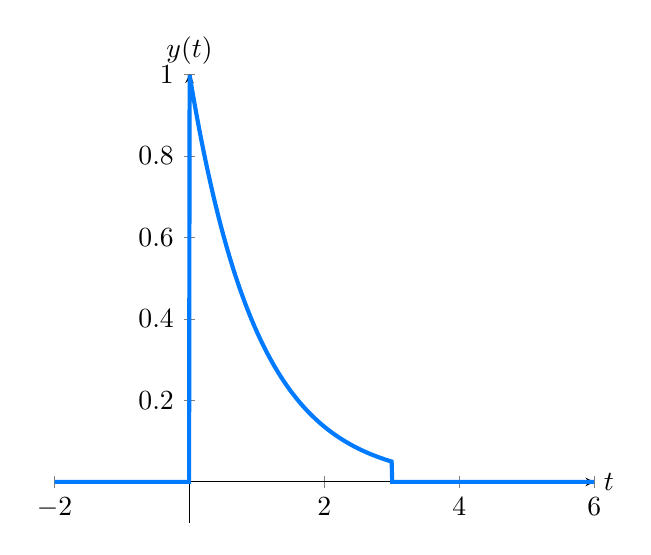
\begin{tikzpicture}
                \begin{axis}[
                    xmin= -2, xmax= 6,
                    ymin= -0.1, ymax = 1,
                    xlabel={$t$}, ylabel={$y(t)$},
                    axis lines = middle,
                    xlabel style={at={(axis cs:6,0)}, anchor=west},
                    ylabel style={at={(axis cs:0,1)}, anchor=south},
                ]
                    \addplot[domain=-2:6, samples=1000, lightblue, line width=1.5] {x<0 ? 0 : (x<3 ? e^(-x) : 0)};
                \end{axis}
            \end{tikzpicture}
        \end{center}
    \item Determinación del valor de $A$

        Comparando con la forma dada  $y(t)=Ae^{-t} $ para $0\le t<3$, se concluye que: \[
        A=1.
        \] 
\end{enumerate}
\item \lb{Sea un sistema discreto $S_1$ con respuesta al impulso $h[n]=\left( \dfrac{1}{5} \right) ^nu[n]$.}
    \begin{enumerate}[label=\color{red}\textbf{\alph*)}]
        \item \db{Determine el número real $A$ tal que  $h[n]-Ah[n-1]=\delta[n]$.}

            El sistema $S_1$ tiene una respuesta al impulso: \[
                h[n]=\left( \dfrac{1}{5} \right) ^nu[n],
            \] donde $u[n]$ es la función escalón unitario, que es igual a 1 para  $n\ge 0$ y $0$ para $n<0$.

            Queremos encontrar un valor de  $A$ tal que: \[
                h[n]-Ah[n-1]=\delta[n],
            \] donde $\delta[n]$ es de la delta de Dirac discreta, que es igual a 1 para  $n=0$ y 0 para  $n\neq 0$.

            \textbf{Sustitución de $h[n]$ y  $h[n-1]$:}

            Sustituyendo $h[n]=\left( \dfrac{1}{5} \right) ^nu[n]$ y $h[n-1]=\left( \dfrac{1}{5} \right) ^{n-1}u[n-1]$, tenemos: \[
                h[n]-Ah[n-1]=\left( \dfrac{1}{5} \right) ^nu[n]-A\left( \dfrac{1}{5} \right) ^{n-1}u[n-1].
            \] 
            \begin{itemize}[label=\textbullet]
                \item \textbf{Caso $n=0$:}

                    Para $n=0,u[0]=1$ y  $u[-1]=0$. Por lo tanto:  \[
                        h[0]-Ah[-1]=\left( \dfrac{1}{5} \right) ^0 -A\cdot 0=1.
                    \] 
                    Esto coincide con $\delta[0]=1$.
                \item  \textbf{Caso $n>0$:}

                    Para $n>0,u[n]=1$ y $u[n-1]=1$. Sustituyendo:  \[
                        h[n]-Ah[n-1]=\left( \dfrac{1}{5} \right) ^n-A\left( \dfrac{1}{5} \right) ^{n-1}=\left( \dfrac{1}{5} \right) ^{n-1}\left( \dfrac{1}{5}-A \right) .
                    \] 
                    Para que esto sea igual a $\delta[n]$, que es 0 para  $n>0$, necesitamos que:  \[
                    \dfrac{1}{5}-A=0\longrightarrow A=\dfrac{1}{5}.
                    \] 

            \end{itemize}
        \item \db{A partir del resultado del apartado anterior, determine la respuesta al impulso del sistema inverso de $S_1$.} 

            El sistema inversor de $S_1$ es aquel cuya respuesta al impulso $h_{\text{inv}}[n]$ satisface: \[
                h_{\text{inv}}[n]\ast h[n]=\delta[n],
            \] donde $\ast$ denota la convolución discreta.

             \textbf{Relación obtenida en el apartado (a):}

             Del apartado (a), sabemos que: \[
                 h[n]-\dfrac{1}{5}h[n-1]=\delta[n].
             \] 
             Esto se puede interpretar como una ecuación en diferencias que describe el sistema inverso. Reescribimos la ecuación como: \[
                 h[n]=\delta[n]+\dfrac{1}{5}h[n-1].
             \] 
             Esta ecuación describe un sistema recursivo, y su solución es la respuesta al impulso del sistema inverso.

             \textbf{Forma explícita de $h_{\text{inv}}[n]$:} 

             La ecuación en diferencias se puede resolver iterativamente. Para $n=0$, tenemos:  \[
                 h[0]=\delta[0]=1.
             \] 
             Para $n=1$, tenemos:  \[
                 h[1]=\dfrac{1}{5}h[0]=\dfrac{1}{5}
             \] 
             Para $n=2$, tenemos:  \[
                 h[2]=\dfrac{1}{5}h[1]=\dfrac{1}{5}\cdot \dfrac{1}{5}=\left( \dfrac{1}{5} \right) ^2.
             \] 
             En general, para $n\ge 0$: \[
                 h_{\text{inv}}[n]=\left( \dfrac{1}{5} \right) ^nu[n].
             \] 
             \begin{center}
                 \begin{tikzpicture}
                     \begin{axis}[
                         xmin= -5, xmax= 5,
                         ymin= -0.1, ymax = 1,
                         xlabel={$n$}, ylabel={$h_{\text{inv}}[n]$},
                         axis lines = middle,
                         xlabel style={at={(axis cs:5,0)}, anchor=west},
                         ylabel style={at={(axis cs:0,1)}, anchor=south},
                     ]
                         \pgfmathsetmacro{\mysamples}{5-(-5)+1}
                         \addplot+[ycomb, mark=*, lightblue, line width=1.5, domain=-5:5, samples=\mysamples] {x<0 ? 0 : (1/5)^x};
                     \end{axis}
                 \end{tikzpicture}
             \end{center}
    \end{enumerate}
\item \lb{Sea la conexión en cascada de dos sistemas $S_1$ y $S_2$ LTI causal tal que:\\
    En $S_1$ la relación entre entrada $x[n]$ y salida  $w[n]=\dfrac{1}{2}w[n-1]+x[n]$.\\
En $S_2$ la relación entre entrada $w[n]$ y salida  $y[n]$ es  $y[n]=\alpha y[n-1]+\beta w[n]$.\\ Si la ecuación en diferencias que relaciona $y[n]$ y  $x[n]$ es  \[
    y[n]=-\dfrac{1}{8}y[n-2]+\dfrac{3}{4}y[n-1]+x[n]
\] } 
\begin{enumerate}[label=\color{red}\textbf{\alph*)}]
    \item \db{Determine $\alpha$ y $\beta$.}

        Se tienen los dos sistemas en cascada:
        \begin{itemize}[label=\textbullet]
            \item En $S_1$ la relación es \[
                    w[n]=\dfrac{1}{2}w[n-1]+x[n].
            \] 
            \item En $S_2$ la relación es \[
                    y[n]=\alpha y[n-1]+\beta w[n].
            \] 
        \end{itemize}
        Como se conectan en cascada, la salida de $S_1$ alimenta a $S_2$. Entonces, sustituyendo la salida de $S_1$ en la ecuación de $S_2$ tenemos: \[
            y[n]=\alpha y[n-1]+\beta\left( x[n]+\dfrac{1}{2}w[n-1] \right) .
        \] 
        Ahora, notamos que la misma relación de $S_2$ aplicada en el instante $n-1$ da: \[
            y[n-1]=\alpha y[n-2]+\beta w[n-1],
        \] de donde se despeja: \[
        w[n-1]=\dfrac{1}{\beta}\left( y[n-1]-\alpha y[n-2] \right) .
        \] 
        Sustituyendo esta expresión en la ecuación de $y[n]$ se tiene:  \[
        \begin{aligned}
            y[n] &=  \alpha y[n-1]+\beta x[n]+\dfrac{\beta}{2}w[n-1] \\
                 &= \alpha y[n-1]+\beta x[n]+\dfrac{\beta}{2}\cdot \dfrac{1}{\beta}\left( y[n-1]-\alpha y[n-2] \right)  \\
                 &= \left( \alpha+\dfrac{1}{2} \right) y[n-1]-\dfrac{\alpha}{2}y[n-2]+\beta x[n]. \\
        \end{aligned}
        \] 
        Pero se nos dice que la ecuación de diferencias global es: \[
            y[n]=\dfrac{3}{4}y[n-1]-\dfrac{1}{8}y[n-2]+x[n].
        \] 
        Al equiparar coeficientes obtenemos: 
        \begin{itemize}[label=\textbullet]
            \item Para $y[n-1]$:  \[
            \alpha+\dfrac{1}{2}=\dfrac{3}{4}\longrightarrow \alpha=\dfrac{3}{4}-\dfrac{1}{2}=\dfrac{1}{4}.
            \] 
        \item Para $y[n-2]$ : \[
        -\dfrac{\alpha}{2}=-\dfrac{1}{8}\longrightarrow \alpha=\dfrac{1}{4}\quad \text{(confirmado).}
        \] 
    \item Para $x[n]$:  \[
    \beta=1.
    \] 
        \end{itemize}
        Por lo tanto, se tiene que: \[
        \bboxed{\alpha=\dfrac{1}{4}\quad\text{ y }\quad \beta=1.} 
        \] 
    \item \db{Obtenga la respuesta al impulso de la conexión en cascada de $S_1$ y $S_2$.} 

        Primero se obtiene la respuesta al impulso de cada sistema individual:
        \begin{itemize}[label=\textbullet]
            \item \textbf{Sistema $S_1$:}

                La ecuación de diferencias es \[
                    w[n]-\dfrac{1}{2}w[n-1]=x[n].
                \] 
                Con entrada impulso $x[n]=\delta[n]$ y siendo el sistema causal, la respuesta al impulso es:  \[
                    h_1[n]=\left( \dfrac{1}{2} \right) ^n u[n],
                \] donde $u[n]$ es la función escalón unitario.
            \item \textbf{Sistema $S_2$:}

                Con $\alpha=\dfrac{1}{4}$ y $\beta=1$, la ecuación es  \[
                    y[n]-\dfrac{1}{4}y[n-1]=w[n].
                \] 
                Para entrada impulso $w[n]=\delta[n]$ se tiene la respuesta:  \[
                    h_2[n]=\left( \dfrac{1}{4} \right) ^nu[n].
                \] 
                Al conectar en cascada, la respuesta total es la convolución de las respuestas individuales: \[
\begin{aligned}
                    h[n]&=h_1[n]\ast h_2[n]=\sum_{k=0}^{n} h_1[k]h_2[n-k]=\sum_{k=0}^{n} \left( \dfrac{1}{2} \right) ^k\left( \dfrac{1}{4} \right) ^{n-k}\\
&=\left( \dfrac{1}{4} \right) ^n \sum_{k=0}^{n} \left( \dfrac{\frac{1}{2} }{\frac{1}{4} } \right) ^k=\left( \dfrac{1}{4} \right) ^n \sum_{k=0}^{n} 2^k =\left( \dfrac{1}{4} \right) ^n\left( 2^{n+1}-1 \right).
\end{aligned}
                \]
                Alternativamente, se puede escribir la respuesta al impulso en forma factorizada: \[
                \bboxed{h[n]=2\left( \dfrac{1}{2} \right) ^n-\left( \dfrac{1}{4} \right) ^n,\quad n\ge 0.}
                \] 
                \begin{center}
                    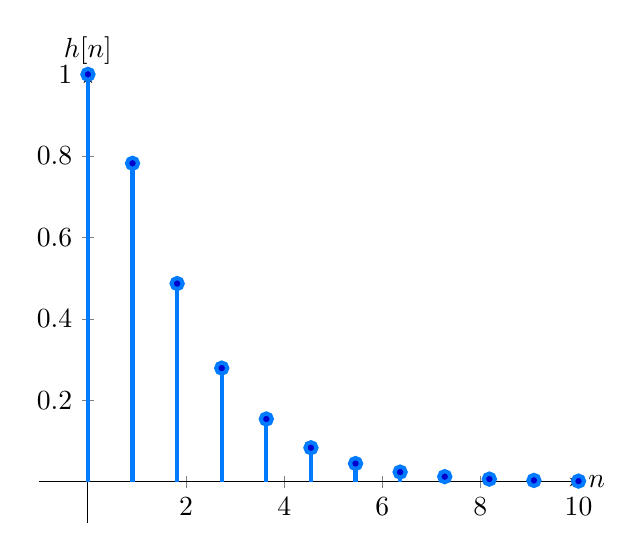
\begin{tikzpicture}
                        \begin{axis}[
                            xmin= -1, xmax= 10,
                            ymin= -0.1, ymax = 1,
                            xlabel={$n$}, ylabel={$h[n]$},
                            axis lines = middle,
                            xlabel style={at={(axis cs:10,0)}, anchor=west},
                            ylabel style={at={(axis cs:0,1)}, anchor=south},
                        ]
                            \pgfmathsetmacro{\mysamples}{10-(-1)+1}
                            \addplot+[ycomb, mark=*, lightblue, line width=1.5, domain=0:10, samples=\mysamples] {2*(1/2)^x-(1/4)^x};
                        \end{axis}
                    \end{tikzpicture}
                \end{center}
        \end{itemize}
\end{enumerate}
\item \lb{La salida de un sistema viene dada por $y[n]=x[2+n]+x[2-n]$.}
    \begin{enumerate}[label=\color{red}\textbf{\alph*)}]
        \item \db{Indique razonadamente si el sistema cumple las propiedades de memoria, causalidad, estabilidad, invarianza en el tiempo y/o linealidad.}

            Analicemos las propiedades:
            \begin{enumerate}[label=\textbf{\arabic*)}]
                \item \textbf{Memoria}

                    Un sistema tiene memoria si su salida depende de valores pasados o futuros de la entrada. En este caso, $y[n]$ depende de  $x[2+n]$ (futuro) y $x[2-n]$ (pasado). Por lo tanto, el sistema  \textbf{tiene memoria}.
                \item \textbf{Causalidad}

                    Un sistema es causal si su salida en el instante $n$ depende únicamente de valores presentes o pasados de la entrada. Aquí, $y[n]$ depende de  $x[2+n]$, que corresponde a valores futuros de la entrada. Por lo tanto, el sistema  \textbf{no es causal}.
                \item \textbf{Estabilidad}

                    Un sistema es estable si, para cualquier entrada acotada, la salida también es acotada. Si $x[n]$ es acotada, entonces  $x[2+n]$ y  $x[2-n]$ también son acotadas, y su suma también será acotada. Por lo tanto, el sistema  \textbf{es estable}. 
                \item \textbf{Invarianza en el tiempo}

                    Un sistema es invariante en el tiempo si un desplazamiento en la entrada produce el mismo desplazamiento en la salida. Supongamos que desplazamos la entrada $x[n]$ por  $k$, es decir, consideramos  $x_k[n]=x[n-k]$. La salida correspondiente sería:  \[
                        y_k[n]=x_k[2+n]+x_k[2-n]=x[2+n-k]+x[2-n-k].
                    \] 
                    Comparando con la salida original $y[n]=x[2+n]+x[2-n]$, vemos que el desplazamiento no se refleja de manera uniforme en la salida. Por lo tanto, el sistema  \textbf{no es invariante en el tiempo}. 
                \item \textbf{Linealidad}
                    
                    Un sistema es lienal si satisface el principio de superposición. Supongamos que las entradas son $x_1[n]$ y $x_2[n]$, con salidas $y_1[n]$ y $y_2[n]$, respectivamente. Si la entrada es una combinación lineal $ax_1[n]+bx_2[n]$, la salida será: \[
                        y[n]=ax_1[2+n]+ax_1[2-n]+bx_2[2+n]+bx_2[2-n].
                    \] 
                    Esto es equivalente a $ay_1[n]+by_2[n]$. Por lo tanto, el sistema \textbf{es lineal.} 
            \end{enumerate}
        \item \db{Considere la señal $x[n]=\bigwedge\left( \dfrac{n}{3} \right) +\bigwedge\left( \dfrac{n-6}{3} \right) $. Obtenga y represente la parte par $x[n]$, indicando si se trata de una señal definida en energía o en potencia.}

            La señal dada es: \[
                x[n]=\bigwedge\left( \dfrac{n}{3} \right) +\bigwedge\left( \dfrac{n-6}{3} \right) ,
            \] donde $\bigwedge(x)$ es el pulso triangular definido como:  \[
            \bigwedge(x)=\begin{cases}
                1-|x|, & |x|<1\\
                0, & \text{en otro caso}
            \end{cases}
            \] 
            \textbf{Parte par de una señal} 

            La parte par de una señal $x[n]$ se define como:  \[
                x_{\text{par}}[n]=\dfrac{x[n]+x[-n]}{2}.
            \] 
            Sustituyendo $x[n]$ en esta fórmula:  \[
                x_{\text{par}}[n]=\dfrac{\bigwedge\left( \frac{n}{3} \right) +\bigwedge\left( \frac{n-6}{3}  \right) +\bigwedge\left( \frac{-n}{3}  \right) +\bigwedge\left( \frac{-n-6}{3}  \right) }{2}.
            \] 
            Ahora evaluamos cada término: 
            \begin{itemize}[label=\textbullet]
                \item $\bigwedge\left( \dfrac{-n}{3} \right) =\bigwedge\left( \dfrac{n}{3} \right) $, ya que el pulso triangular es par.
                \item $\bigwedge\left( \dfrac{-n-4}{3} \right) =\left( \dfrac{-(n+6)}{3} \right) =\bigwedge\left( \dfrac{n+6}{3} \right) $, ya que el pulso traingular también es par.
            \end{itemize}
            Por lo tanto: \[
                x_{\text{par}}[n]=\dfrac{\bigwedge\left( \frac{n}{3}  \right) +\bigwedge\left( \frac{n-6}{3}  \right) +\bigwedge\left( \frac{n}{3}  \right) +\bigwedge\left( \frac{n+6}{3}  \right) }{2}=\bigwedge\left( \dfrac{n}{3} \right) +\dfrac{\bigwedge\left( \frac{n-6}{3}  \right) +\bigwedge\left( \frac{n+6}{3}  \right) }{2}.
            \] 
            \textbf{Señal definida en energía o potencia}

            Para determinar si la señal está definida en energía o en potencia, calculamos la energía total: \[
                E=\sum_{n=-\infty}^{\infty} |x[n]|^2.
            \] 
            Dado que $\bigwedge(x)$ tiene soporte finito,  $x[n]$ también tiene soporte finito, lo que implica que la energía es finita. Por lo tanto,  $x[n]$ es una señal  \textbf{definida en energía}. 
        \item \db{Realice la convolución discreta $x_1[n]\ast x_2[n]$, siendo \[
        \begin{array}{c}
            x_1[n]=\prod\left( \dfrac{n-6}{13} \right) +u[n-13]\\
            x_2[n]=\bigwedge\left( \dfrac{n-3}{5} \right) .
        \end{array}
        \] } 
    \end{enumerate}
\item \lb{Se pretende filtrar la señal $x(t)$ con un sistema LTI cuya respuesta al impulso es $h(t)$. \[
\begin{array}{c}
    x(t)=\left( 1+\bigwedge\left( \dfrac{t-4}{1} \right)  \right) \prod\left( \dfrac{t-1.5}{5} \right) \\
    h(t)=\dfrac{9}{2}\bigwedge\left( \dfrac{t-4}{3} \right) u(t-5)+2\delta(t)
\end{array}
\] } 
\begin{enumerate}[label=\color{red}\textbf{\alph*)}]
    \item \db{Represente detalladamente las señales $x(t)$ y $h(t)$.}

    \begin{center}
        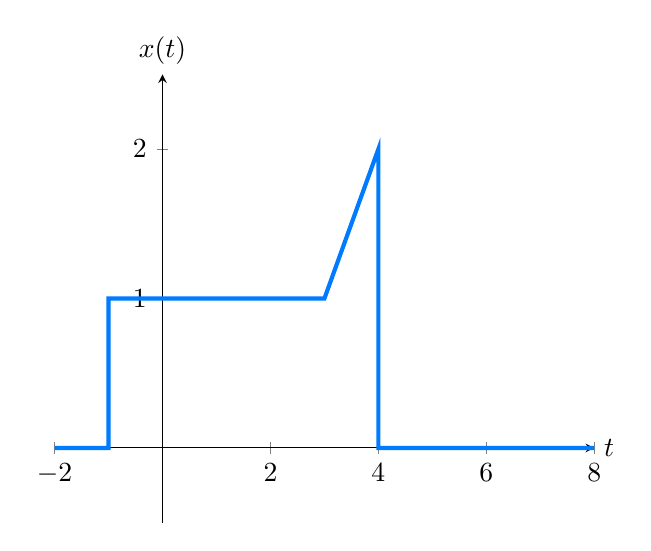
\begin{tikzpicture}
            \begin{axis}[
                xmin= -2, xmax= 8,
                ymin= -0.5, ymax = 2.5,
                xlabel={$t$}, ylabel={$x(t)$},
                axis lines = middle,
                xlabel style={at={(axis cs:8,0)}, anchor=west},
                ylabel style={at={(axis cs:0,2.5)}, anchor=south},
            ]
            \addplot[lightblue, line width=1.5] coordinates {
                    (-2,0) (-1,0) (-1,1) (3,1) (4,2) (4,0) (8,0)
                };
            \end{axis}
        \end{tikzpicture}\qquad
        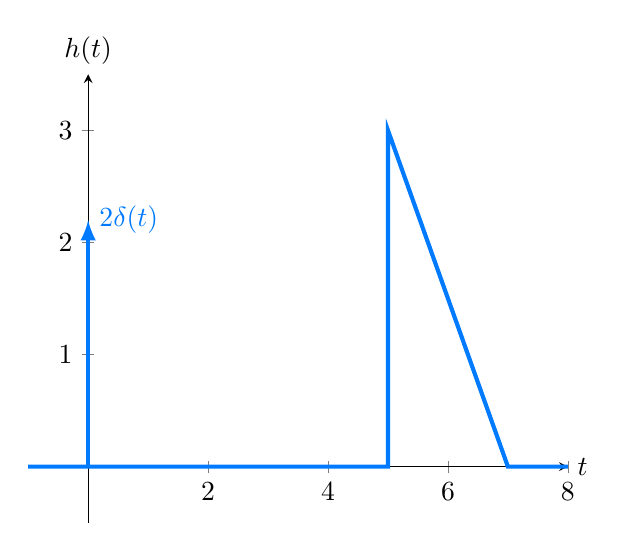
\begin{tikzpicture}
            \begin{axis}[
                xmin= -1, xmax= 8,
                ymin= -0.5, ymax = 3.5,
                xlabel={$t$}, ylabel={$h(t)$},
                axis lines = middle,
                xlabel style={at={(axis cs:8,0)}, anchor=west},
                ylabel style={at={(axis cs:0,3.5)}, anchor=south},
            ]
            \addplot[lightblue, line width=1.5] coordinates {
                    (-1,0) (5,0) (5,3) (7,0) (8,0)
                };
            \draw[-latex, lightblue, line width=1.5] (axis cs:0,0) -- (axis cs:0,2.2) node[right] {$2\delta(t)$};
            \end{axis}
        \end{tikzpicture}
    \end{center}
    \item \db{Indique razonadamente si el sistema definido por $h(t)$ cumple las propiedades de memoria, causalidad, estabilidad y/o invarianza.}

        Considerando $h(t)\dfrac{9}{2}\bigwedge\left( \dfrac{t-4}{3} \right) u(t-5)+2\delta(t)$, se pueden señalar las siguientes propiedades:
        \begin{itemize}[label=\textbullet]
            \item \textbf{Memoria:}

                Un sistema es \textit{sin memoria} si la salida en cada instante depende únicamente de la entrada en ese instante. En los sistemas LTI, esto ocurre solmanete si $h(t)=K\delta(t)$ (un escalamiento instantáneo). EN este caso, al existir además la componente continua (la parte triangular para $t\ge 5$), la salida depende de valores previos o posteriores de la entrada. Por ello, el sistema \textbf{tiene memoria}.
            \item \textbf{Causalidad:}

                Un sistema causal requiere que $h(t)=0$ para  $t<0$. Aquí:
                 \begin{itemize}[label=\textbullet]
                    \item El término $2\delta(t)$ tiene soporte en  $t=0$.
                    \item La función  $u(t-5)$ obliga a que el pulso triangular sea 0 para $t<5$. Por lo tanto,  $h(t)=0$ para  $t<0$ y el sistema  \textbf{es causal}. 
                \end{itemize}
            \item \textbf{Estabilidad:}

                La estabilidad exige que la integral del valor absoluto de la respuesta al impulso sea finita: \[
                \int_{-\infty}^{\infty} |h(t)|\dt<\infty. 
                \] 
                La delta aporta una integral igual a 2, y la parte triangular tiene soporte acotado $(t\in [5,7])$ y está escalada por $\dfrac{9}{2}$, de modo que su integral es finita. Por ello, el sistema \textbf{es estable}.
            \item \textbf{Invarianza en el tiempo:}

                Dado que la respuesta al impulso $h(t)$ define al sistema LTI, éste es, por construcción, \textbf{invariante en el timepo}. 
        \end{itemize}
    \item \db{Calcule de forma analítica la convolución $y(t)=x(t)\ast h(t)$. (\underline{Nota:} puede hacer uso de las propiedades de la convolución).}

        Se desea calcular $$y(t)=(x\ast h)(t)=\int_{-\infty}^{\infty} x(\tau)h(t-\tau)\mathrm{d}\tau. $$

        Debido a la linealidad de la convolución y a la estructura de $h(t)$, escribimos  \[
        y(t)=x(t)\ast\left[ 2+d(t) \right] +x(t)\ast\left[ \dfrac{9}{2}\bigwedge\left( \dfrac{t-4}{3} \right) u(t-5) \right] =2x(t)+\dfrac{9}{2}\int_{-\infty}^{\infty} x(\tau) \bigwedge\left( \dfrac{t-\tau-4}{3} \right) u(t-\tau-5)\mathrm{d}\tau.
        \] 
        \textbf{Observaciones para simplificar la integral:}
        \begin{itemize}[label=\textbullet]
            \item El escalón $u(t-\tau-5)$ exige que  $t-\tau\ge 5$, es decir, $\tau\le t-5$.
            \item La función $\bigwedge\left( \dfrac{t-\tau-4}{3} \right) $ es diferente de cero únicamente cuando \[
                    \left| \dfrac{t-\tau-4}{3} \right| \le 1\longrightarrow t-\tau\in [4,7].
            \] 
            \item Combinando los dos puntos anteriores se tiene que el integrando es no nulo cuando: \[
                t-\tau\in [5,7]\longrightarrow \tau\in [t-7,t-5].
        \] 
            \item Además, recordemos que $x(\tau)$ es no nula únicamente en  $\tau\in [-1,4]$.
        \end{itemize}
        Por lo tanto, el intervalo efectivo de integración es \[
            \delta\in\left[ \max \{-1,t-7\}, \min \{4,t-5\}  \right] .
        \] 
        En este intervalo (donde además se cumple que $t-\tau\in [5,7]$), se tiene que \[
        \bigwedge\left( \dfrac{t-\tau-4}{3} \right) =1-\dfrac{t-\tau-4}{3}.
        \] 
        Entonces la convolución se puede escribir de forma compacta como \[
            \boxed{y(t)=2x(t)+\dfrac{9}{2}\int_{\max \{-1,t-7\} }^{\min \{4,t-5\} } x(\tau)\left[ 1-\dfrac{t-\tau-4}{3} \right] \mathrm{d}\tau. }
        \] 
        La señal $x(t)$ se define como  \[
        x(t)=\left( 1+\bigwedge\left( \dfrac{t-4}{1} \right)  \right) \prod\left( \dfrac{t-1.5}{5} \right) .
        \] 
        Recordemos que el pulso rectangular \[
        \prod\left( \dfrac{t-1.5}{5} \right) 
        \] toma el valor 1 cuando \[
        \left| \dfrac{t-1.5}{5} \right| \le \dfrac{1}{2}\longrightarrow |t-1.5|\le 2.5\longrightarrow t\in [1.5-2.5,1.5+2.5]=[-1,4],
        \] y 0 en otro caso.

        La función triangular \[
        \bigwedge\left( \dfrac{t-4}{1} \right) 
        \] tiene soporte cuando \[
        \left| \dfrac{t-4}{1} \right| \le 1\longrightarrow t\in [4-1,4+1]=[3,5],
        \] y se define como \[
        \bigwedge\left( \dfrac{t-4}{1} \right) =\begin{cases}
            1-|t-4|, & t\in [3,5]\\
            0, & \text{en otro caso}
        \end{cases}
        \] 
        Por lo tanto, la parte de $x(t)$ que esté "dentro" del rectángulo (es decir, para $t\in [-1,4]$) se tiene:
        \begin{itemize}[label=\textbullet]
            \item  Si $t$ está fuera del intervalo $[3,5]$ (es decir, para $t\in [-1,3)$) el pulso triangular es 0 y entonces \[
            x(t)=1+0=1.
            \] 
        \item Si $t\in [3,4]$ (recordando que el rectángulo está definido solo hasta $t=4$) el pulso triangular es no nulo y, usando que para estos $t$ se tiene  $|t-4|=4-t$, se obtiene  \[
        x(t)=1+\left[ 1-(4-t) \right] =t-2.
        \] 
        \end{itemize}
        En resumen: \[
        x(t)=\begin{cases}
            1, & t\in [-1,3)\\
            t-2, & t\in [3,4]\\
            0, & \text{en otro caso}
        \end{cases}
        \] 
        Esta expresión define completamente a $y(t)$, cuyo soporte se extiende (por las propiedades de la convolución) aproximadamente para $t\in [4,11]$. En particular, para $t<4$ la condición  $\tau\le t-5$ no es compatible con el soporte de $x(\tau)$ (ya que $t-5<-1$) y por lo tanto el término de la integral se anula, de donde $y(t)=2x(t)$ en esos instantes.
    \item \db{Calcule la energía y la potencia de $x(t)$, indicando si se trata de una señal definida en energía o en potencia.} 

        La energía de $x(t)$ se define como  \[
        E_x=\int_{-\infty}^{\infty} |x(t)|^2\dt. 
        \] 
        Como $x(t)$ es no nula únicamente en  $t\in [-1,4]$, se puede separar la integral en dos partes:
        \begin{itemize}[label=\textbullet]
            \item Para $t\in [-1,3]$ se tiene $x(t)=1$, de modo que  \[
                \int_{-1}^{3} 1^2\dt=3-(-1)=4. 
                \] 
            \item Para $t\in [3,4]$ se tiene $x(t)=t-2$; por lo tanto  \[
            \int_{3}^{4} (t-2)^2\dt=\left\{ \begin{array}{l}
                u=t-2\\
                \text{Si }t=3\longrightarrow t=1\\
                \text{Si }t=4\longrightarrow t=2
            \end{array} \right\} =\int_{1}^{2} u^2\du =\left[ \dfrac{u^3}{3} \right] _1^2=\dfrac{8-1}{3}  =\dfrac{7}{3}.
            \] 
        \end{itemize}
        En conjunto, \[
        E_x=4+\dfrac{7}{3}=\dfrac{19}{3}.
        \] 
        La potencia media de $x(t)$ viene dada por  \[
        P_x=\lim_{T \to \infty} \dfrac{1}{2T}\int_{-T}^{T} |x(t)|^2\dt=\lim_{T \to \infty} \dfrac{E_x}{2T}=\dfrac{\frac{19}{3} }{\infty}=0.  
        \] 
        Por lo tanto, $x(t)$ es una \textbf{señal definida en energía}.
\end{enumerate}
\item \lb{Considere un sistema LTI cuya señal de salida $y(t)$ viene dada por \[
y(t)=\int_{1}^{\infty} 3e^{-(2+5j)\tau}x(t-\tau)\mathrm{d}\tau.  
\] } 
\begin{enumerate}[label=\color{red}\textbf{\alph*)}]
    \item \db{Obtenga la respuesta al impulso del sistema LTI.}

        Recordemos que para un sistema LTI la salida se expresa como \[
        y(t)=\int_{-\infty}^{\infty} h(\tau)x(t-\tau)\mathrm{d}\tau. 
        \] 
        En el enunciado se tiene \[
        y(t)=\int_{1}^{\infty} 3e^{-(2+5j)\tau}x(t-\tau)\mathrm{d}\tau,  
        \] lo cual implica que la función $h(\tau)$ del sistema es:  \[
        \begin{array}{c}
            h(\tau)=3e^{-(2+5j)\tau}\quad \text{para }\tau\ge 1,\\
            h(\tau)=0\text{ para }\tau<1.
        \end{array}
        \] 
        Utilizando la función escalón unitario $u(\cdot )$, podemos escribir de forma compacta: \[
            \boxed{h(t)=3e^{-(2+4j)t}u(t-1). }
        \] 
    \item \db{Indique razonadamente si el sistema posee las propiedades de memoria, causalidad y/o estabilidad.}
        \begin{itemize}[label=\textbullet]
            \item \textbf{Memoria:}

                Un sistema es sin memoria cuando la salida en el tiempo $t$ depende únicamente de  $x(t)$. Dado que en la convolución la salida depende de  $x(t-\tau)$ para  $\tau\ge 1$, la salida depende de valores pasados de la entrada. Por lo tanto, el sistema tiene memoria.
            \item \textbf{Causalidad:}

                Para que un sistema sea causal es necesario que la respuesta al impulso sea nula para tiempos negativos, es decir, $h(t)=0$ para $t<0$. En nuestro caso,  $h(t)=0$ para  $t<1$, de modo que la salida en  $t$ depende únicamente de valores de entrada en tiempos anteriores. Así, el sistema es causal.
            \item \textbf{Estabilidad:}

                Un sistema es estable si: \[
                \int_{-\infty}^{\infty} |h(t)|\dt<\infty. 
                \] 
                Dado que \[
                |h(t)|=3e^{-2t} \text{ para } t\ge 1,
                \] se tiene \[
                \int_{-\infty}^{\infty} |h(t)|\dt=\int_{1}^{\infty} 3e^{-2t}\dt=3\left[ \dfrac{e^{-2t} }{-2} \right]_1^\infty=\dfrac{3}{2}e^{-2}<\infty.
            \] 
            Por lo tanto, el sistema es estable.
        \end{itemize}
    \item \db{Calcule la señal de salida del sistema cuando la señal de entrada es un escalón unitario.}

        Sea $x(t)=u(t)$. Entonces a salida es:  \[
        y(t)=\int_{1}^{\infty} 3e^{-(2+5j)\tau}u(t-\tau)\mathrm{d}\tau.  
        \] 
        La función  $u(t-\tau)$ vale 1 cuando  $t-\tau\ge 0$ (es decir, $\tau\le t$) y 0 en caso contrario. Se distinguen dos casos:
        \begin{itemize}[label=\textbullet]
            \item Para $t<1$:

                Debido a que  $\tau\ge 1$ en la integración y además $t<1$ implica  $\tau>t$, se tiene  $u(t-\tau)=0$ para todo  $\tau$ en el intervalo de integración. Por ello,  \[
                y(t)=0,\quad t<1.
                \] 
            \item Para $t\ge 1$:

                La variable de integración varía de $\tau=1$ hasta  $\tau=t$ (pues para $\tau>t$ se tiene  $u(t-\tau)=0$). Así, \[
                y(t)=\int_{1}^{t} 3e^{-(2+5j)\tau}\mathrm{d}\tau=3\left[ \dfrac{e^{-(2+5j)\tau} }{-(2+5j)} \right]_{\tau=1}^{\tau=t} =\dfrac{3}{2+5j}\left( e^{-(2+5j)}-e^{-(2+5j)t}   \right)  . 
                \] 
        \end{itemize}
        Resumiendo: \[
            \boxed{y(t)=\begin{cases}
                    0, & t<1,\\
                    \dfrac{3}{2+5j}\left( e^{-(2+5j)}-e^{-(2+5j)t}   \right) , & t\ge 1.
            \end{cases}}
        \] 
    \item \db{Calcule la energía y potencia de la señal $y(t)$, indicando si se trata de una señal definida en energía o en potencia.} 

        Observamos primero el comportamiento de $y(t)$ cuando  $t\to \infty$. Para $t\ge 1,$ \[
        y(t)=\dfrac{3}{2+5j}\left( e^{-(2+5j)}-e^{-(2+5j)t}   \right) .
        \] 
        Dado que \[
        \lim_{t \to \infty} e^{-(2+5j)t}=0, 
        \] obtendremos \[
        \lim_{t \to \infty} y(t)=\dfrac{3}{2+5j}e^{-(2+5j)} =y_\infty.
        \] 
        El valor constante no es cero, lo que implica que la salida tiene una componente permanente.
        \begin{itemize}[label=\textbullet]
            \item \textbf{Energía:}

                La energía de la señal es \[
                E_y=\int_{-\infty}^{\infty} |y(t)|^2\dt. 
                \] 
                Debido a que para $t\ge T$ (con $T$ suficientemente grande) $y(t)$ se aproxima a un valor constante distinto de cero, la integral diverge a infinito. Es decir, \[
                E_y=\infty.
                \] 
            \item \textbf{Potencia:}

                La potencia media se define mediante \[
                P_y=\lim_{T \to \infty} \dfrac{1}{T}\int_{0}^{T} |y(t)|^2\dt. 
                \] 
                Como para $t$ grande  $y(t)\approx y_\infty$ (constante), la potencia resulta ser el cuadrado del módulo del valor asintótitco: Primero, calculemos el módulo:  \[
                \left| \dfrac{3}{2+5j} \right| =\dfrac{3}{\sqrt{2^2+5^2} }=\dfrac{3}{\sqrt{29} },
                \] y \[
                \left| e^{-(2+5j)}  \right| =e^{-2}. 
                \] 
                De modo que \[
                |y_\infty|=\dfrac{3}{\sqrt{29} }e^{-2}. 
                \] 
                Por ello, la potencia es \[
                P_y=|y_\infty|^2=\left( \dfrac{3e^{-2}}{\sqrt{29}}  \right)^2 =\dfrac{9e^{-4} }{29}.
                \] 
        \end{itemize}
        Dado que la energía es infinita y la potencia es finita, concluimos que la señal $y(t)$ es una señal defindia en potencia.
\end{enumerate}

\item \lb{Se pretende filtrar la señal $x[n]$ con un sistema LTI cuya respuesta al impulso es  $h[n]$:  \[
\begin{array}{c}
    x[n]=(u[n+6]-u[n-7]+\delta[-n+7])u[-n+10]\\
    h[n]=0.4^{n-2}u[n-2]u[n]
\end{array}
\] } 
\begin{enumerate}[label=\color{red}\textbf{\alph*)}]
    \item \db{Represente detalladamente $x[n]$ y  $h[n]$.}
    \item \db{Indique razonadamente si el sistema definido por $h[n]$ cumple las propiedades de memoria, causalidad y/o estabilidad.}
    \item \db{Utilizando la definición, calcule la convolución $y[n]=x[n]\ast h[n]$.}
    \item \db{Calcule la energía y la potencia de $x[n]$, indicando si es una señal definida en energía o en potencia.} 
\end{enumerate}
\item \lb{Considere el siguiente diagrama de bloques de un sistema causal (figura 2).}
    \begin{center}
\begin{tikzpicture}[
    block/.style={draw, minimum width=1cm, minimum height=1cm, lightblue},
    sum/.style={draw, circle, minimum size=5mm, inner sep=0pt, lightblue},
    connector/.style={-Latex, thick, lightblue},
    node distance=1.5cm and 1.5cm,
	scale=0.7
]

% Nodos
\node[lightblue] (input) at (0,0) {$x[n]$};
\node[sum, right=1.5cm of input] (sum) {+};
\node[block, below right=0.5cm and 2.2cm of sum] (D1) {$D$};
\node[block, below=1.5cm of D1] (D2) {$D$};
\node[right=7cm of sum, lightblue] (output) {$y[n]$};

% Líneas y conexiones
\draw[connector] (input) -- (sum);

% Bucle superior
\draw[connector] (D1) ++(0,-1.5) -| node[pos=0.25, above] {$\tfrac{1}{2}$} (sum);
\draw[connector] (sum) -| (D1);

% Bucle inferior
\draw[connector] (D1) -- (D2);
\draw[connector] (D2) |- ++(0,-1.5) -| node[above, pos=0.25] {$-3$} ++(4,0) |- (output);

\end{tikzpicture}\\
\lb{Figura 2}
    \end{center}
    \begin{enumerate}[label=\color{red}\textbf{\alph*)}]
        \item \db{Obtenga la ecuación en diferencias con coeficientes constantes que relaciona la señal de entrada $x[n]$ con la señal de salida  $y[n]$.} 
        \item \db{Obtenga la respuesta al impulso del sistema e indique razonadamente si se trata de un sistema FIR o IIR. Justifique si el sistema cumple las propiedades de memoria, causalidad y/o estabilidad.}
        \item \db{Considere la señal de entrada $x[n]=\prod\left( \dfrac{n-2}{5} \right) +u[2n-20]u[-n+14]$. Represente la señal y calcule su energía total y potencia media.}
        \item \db{Determine la señal de salida del sistema $y[n]$ cuando se introduce la señal  $x[n]$ del apartado anterior como señal de entrada.} 
    \end{enumerate}
\item \lb{Considere el sistema descrito por la siguiente relación entre la entrada y la salida: \[
            y[n]=\sum_{k=-\infty}^{n-1} x[k-1]
\] } 
\begin{enumerate}[label=\color{red}\textbf{\alph*)}]
    \item \db{Indique razonadamente si el anterior sistema cumple las propiedades de memoria, causalidad, estabilidad, invertibilidad, linealidad y/o invarianza temporal.}
    \item \db{¿Se trata de un sistema LTI? En caso afirmativo, obtenga y represente su respuesta al impulso $h[n]$.}
    \item \db{Utiliza la definición de convolución, obtenga la salida del sistema del enunciado, $y[n]$, cuando a su entrada se tiene la señal  $x[n]=(n+1)u[n]$.}
    \item \db{Calcule la energía total y la potencia media de la señal $x[n]$ del apartado anterior, indicando de qué tipo de señal se trata según estos valores.} 
\end{enumerate}
\item \lb{Considere el sistema LTI discreto consistente en la conexión en serie de los subsistemas LTI descritos por \[
\begin{array}{c}
    h_1[n]=n\delta[n-1]\\
    h_2[n]=\left( \dfrac{1}{3} \right) ^{n-1}u[n+1]
\end{array}
\] Obtenga la salida del sistema $y[n]$ cuando la entrada es  \[
x[n]=(-1)^{n}(u[2-n]-u[-n-1])
\] } 
\item \lb{Represente el diagrama de bloques en forma canónica del sistema dado por la ecuación diferencial \[
\dfrac{\mathrm{d}^2y(t)}{\dt^2}+2\dfrac{\mathrm{d}y(t)}{\dt}-8y(t)=x(t)-\dfrac{\mathrm{d}x(t)}{\dt}
\] } 
\item \lb{Dibuje el diagrama de bloques de los siguientes sistemas LTI causales descritos mediante sus ecuaciones en diferencias:}
    \begin{enumerate}[label=\color{red}\textbf{\alph*)}]
        \item \db{$y[n]=\dfrac{1}{3}y[n-1]+\dfrac{1}{2}x[n]$} 
        \item \db{$y[n]=\dfrac{1}{3}y[n-1]+x[n-1]$} 
    \end{enumerate}
\item \lb{Dibuje el diagrama de bloques de los siguientes sistemas LTI causales descritos mediante sus ecuaciones diferenciales:}
    \begin{enumerate}[label=\color{red}\textbf{\alph*)}]
        \item \db{$y(t)=-\dfrac{1}{2}\dfrac{\mathrm{d}y(t)}{\dt}+4x(t)$} 
        \item \db{$\dfrac{\mathrm{d}y(t)}{\dt}+3y(t)=x(t)$} 
    \end{enumerate}
\item \lb{Obtenga las formas directas I y II del sistema LTI causal cuya entrada $x[n]$ y salida $y[n]$ están relacionadas mediante la ecuación en diferencias \[
            y[n]=-ay[n-1]+b_0x[n]+b_1x[n-1]
\] } 
\item \lb{Obtenga las formas directas I y II del sistema LTI causal cuya entrada $x(t)$ y salida  $y(t)$ están relacionadas mediante la ecuación diferencial  \[
a_1 \dfrac{\mathrm{d}y(t)}{\dt}+a_0y(t)=b_0x(t)+b_1 \dfrac{\mathrm{d}x(t)}{\dt}
\] } 
\item \lb{Obtenga que la ecuación diferencial del ejercicio anterior se puede escribir en forma de ecuación integral como \[
y(t)=A \int_{-\infty}^{t} y(\tau)\mathrm{d}\tau+Bx(t)+C \int_{-\infty}^{t} x(\tau)\mathrm{d}\tau  
\] expresando las constantes $A,B$ y  $C$ en términos de las constantes $a_0,a_1,b_0$ y $b_1$.\\ Obtenga las formas directas I y II del sistema LTI causal expresado según esta ecuación integral.} 
\end{enumerate}
\end{document}
